% !TEX root = catron-dissertation.tex
% arara: pdflatex
% arara: bibtex
% arara: pdflatex
% arara: pdflatex

\documentclass[twoadvisors,noinfo]{nddiss2e}

\usepackage{graphicx}
\usepackage{subcaption}
\usepackage{csquotes}
\usepackage{epstopdf}
\epstopdfsetup{outdir=./images/}
\usepackage[makeroom]{cancel}
\usepackage{listings}
\usepackage{amsmath}
% \usepackage{fdsymbol}
% \usepackage{physics}
% \usepackage{mathtools}

\lstset
{ %Formatting for code in appendix
    language=Matlab,
    basicstyle=\footnotesize,
    numbers=left,
    stepnumber=1,
    showstringspaces=false,
    tabsize=1,
    breaklines=true,
    breakatwhitespace=false,
}

% Custom Math Objects
\DeclareMathOperator{\fft}{FFT}
\DeclareMathOperator{\fftn}{FFT_n}
\DeclareMathOperator{\fftthree}{FFT_3}
\DeclareMathOperator{\fftshift}{FFT_{SHIFT}}
\DeclareMathOperator{\ifft}{IFFT}
\DeclareMathOperator{\ifftn}{IFFT_n}
\DeclareMathOperator{\wf}{WF}
\DeclareMathOperator{\f}{F}
\DeclareMathOperator{\opd}{OPD}
\DeclareMathOperator{\opdrms}{OPD_{RMS}}
\DeclareMathOperator{\opl}{OPL}
\DeclareMathOperator{\sr}{SR}
\DeclareMathOperator{\spl}{SPL}
\DeclareMathOperator{\real}{REAL}


\begin{document}

\frontmatter

\title{ Filtering of Acoustic Information from Aero-Optical Measurements }
\author{ Brian Lowell Catron }
\work{ Dissertation }
\degaward{ Doctor of Philosophy }
\advisor{ R. Mark Rennie }
\secondadvisor{ Eric J. Jumper}
\department{ Aerospace and Mechanical Engineering}
\maketitle

\copyrightyear{ 2021 }
\makecopyright

\begin{abstract}
 Abstract Goes Here
\end{abstract}

\begin{dedication}
 To my wife Karen \& our son Arthur
\end{dedication}

\tableofcontents
\listoffigures
\listoftables

\begin{symbols}[cl]
% A
\sym{Ap}{Aperture size - Typically diameter}
% B
% C
% D
% E
% F
% G
% H
% I
\sym{I}{Actual on target intensity}
\sym{I_0}{Diffraction-limited intensity}
% J
% K
\sym{k}{Wavenumber ($k=2\pi/\lambda$)}
% L
% M
% N
\sym{n}{Index of refraction}
% O
\sym{\opd}{Optical path difference}
\sym{\opdrms}{Spatial $\opd$ root-mean-square}
% P
% Q
% R
% S
\sym{\sr}{Strehl ratio ($\textrm{SR}=I/I_0$)}
% T
% U
% V
% W
% X
% Y
% Z
\sym{}{\textbf{Greek}}
% ALPHA
% BETA
% GAMMA
% DELTA
\sym{\delta}{Boundary layer thickness}
% EPSILON
% ZETA
% ETA
% THETA
\sym{\left<\theta^2\right>}{Mean-squared of the fluctuating deflection angle}
% IOTA
% KAPPA
% LAMBDA
% MU
% NU
% XI
% OMICRON
% PI
% RHO
% SIGMA
% TAU
% UPSILON
% PHI
% CHI
% PSI
% OMEGA
\end{symbols}


\begin{acknowledge}
\end{acknowledge}

\mainmatter
% !TEX root = catron-dissertation.tex
\epstopdfsetup{outdir=./images/01_introduction/}

\chapter{Introduction}
\label{chap:01_intro}

Directed-energy systems have a variety of uses but typically fall into one of two categories: communications and weapons.
The primary benefits of directed-energy communications is the ability to have secure point-to-point data transfer that is high unlikely to intercept or be interfered with \cite{crs-2021-RwNjGeZD}.
Directed-energy weapons are likely to have a lower cost per shot and a deeper magazine when compared to traditional munitions \cite{crs-2021-hyCUE868}.
As ground based directed-energy systems are slowly rolled out, most prominently aboard the USS Ponce \cite{crs-2021-Atxb7GDv}, there is a desire to field a system aboard an aircraft.

There have been two major attempts to field a directed-energy system aboard an aircraft to date \cite{Jumper-2013-8KtN3pue}.
The first was the Airborne Laser Laboratory (ALL) which took place in the late 1970's and early 1980's which used a CO$_2$ laser at 10.6-$\mu$m.
The second was the Airborne Laser (ABL) program which operated in the 2000's and used a COIL laser at 1.315-$\mu$m.
Airborne optical systems have to deal with a phenomenon know as ``aero-optics,'' which is optical distortions caused by various aero-dynamic flow features.
These optical distortions were first noticed due to image degradation in wind tunnel measurements in the 1950's \cite{Stine-1956-UaRzVZCe} as well as in photo-reconnaissance missions in the 1960's \cite{Kyrazis-2013-vwKeEBym}.

The intensity of that makes through an optical disturbance to a target, $I$, divided by the diffraction-limited performance, $I_0$, is known as the Strehl ratio \cite{Mahajan-1982-kkXM4eaB}, $\sr$,
\begin{equation}
  \sr = \frac{I}{I_0} \textrm{.}
  \label{eqn:01_strehl_ratio_definition}
\end{equation}
The diffraction-limited performance is the intensity that would make it to the same target if not for a disturbance.
The Airborne Laser Laboratory had an estimated Strehl ratio of 95\%\cite{Jumper-2013-8KtN3pue} meaning the ``aero-optics problem'' effectively did not apply.
After the Airborne Laser Laboratory program there was a desire to move toward shorter wavelengths in order to take advantage of improved diffraction-limited performance \cite{Jumper-2001-6QDh7zDy},
\begin{equation}
  \frac{I_0}{P} = \frac{1}{\pi}\left(\frac{Ap}{\lambda z}\right)^2 \textrm{,}
  \label{eqn:01_farfield_intensity}
\end{equation}
where $P$ is the laser output power, $Ap$ is the aperture size, and $z$ is the propagation distance.
This improved diffraction-limited performance is shown in Figure \ref{fig:01_farfield_intensity}.
\begin{figure}
  \centering
  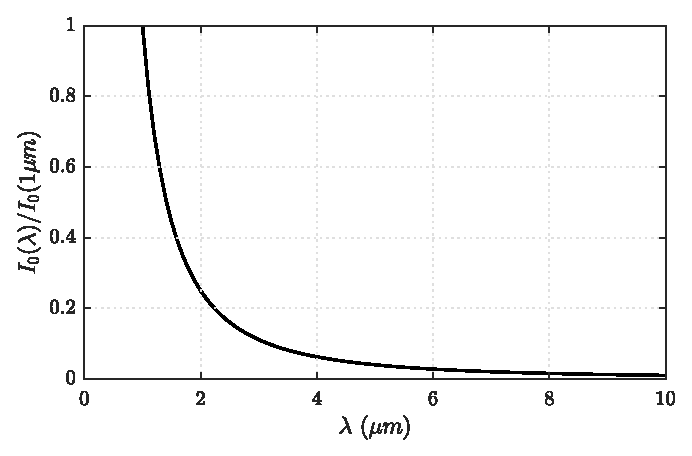
\includegraphics{../matlab/01_introduction/farfield_intensity.eps}
  \caption{Diffraction-limited far-field intensity of a beam normalized by the performance at 1-$\mu$m.}
  \label{fig:01_farfield_intensity}
\end{figure}
By only changing the laser source from a 10-$\mu$m to 1-$\mu$m wavelength the diffraction-limited performance can be increased 100 times.

Aero-optical issues start to become apparent as the wavelength is decreased as is evident by the Mar\'echal approximation \cite{Mahajan-1983-hg7ahvJM} which relates the Strehl ratio to wavelength,
\begin{equation}
  \sr \approx \exp\left\{-\left[\frac{2\pi \opdrms}{\lambda}\right]^2\right\} \textrm{,}
  \label{eqn:01_strehl_ratio}
\end{equation}
where $\opdrms$ is the spatial root-mean-square of the optical path difference over the aperture and is a way to quantify the optical disturbance that will be discussed in Chapter \ref{chap:02_lit_review}.
If the ALL system's laser was swapped with another laser of a lower wavelength, the Strehl ratio would significantly decrease as shown by Figure \ref{fig:01_strehl_ratio}.
\begin{figure}
  \centering
  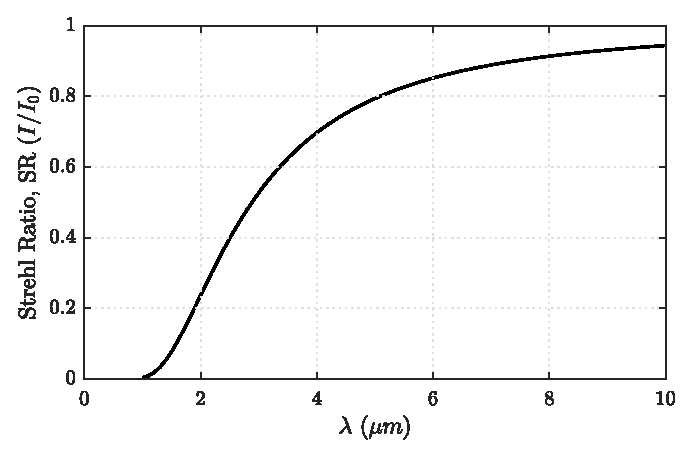
\includegraphics{../matlab/01_introduction/strehl_ratio.eps}
  \caption{Strehl ratio due to the $\opdrms$ of the Airborne Laser Laboratory (ALL) at various laser wavelengths.  ALL had an estimated Strehl ratio of 95\% with its 10.6-$\mu$m laser.}
  \label{fig:01_strehl_ratio}
\end{figure}
While the hypothetical case of going from 10 to 1-$\mu$m resulted in a 100-fold increase in diffraction-limited performance, the actual on-target intensity that this hypothetical system obtains would be essentially zero.
This means that the aero-optical problem can no longer be ignored and was recognized as one of the main developmental risks of the ABL program \cite{DOTE-1999-HnkadUEw}.
{\color{red}{Do you have or know of a source that at the very least alludes to the aero-optical issues with ABL that greatly limited its field of regard?}}

As the next generation of airborne directed-energy systems are developed some amount of ground testing of those systems will need to occur.
In order to understand the aero-optical environment that these systems will experience in the air wind tunnel tests will need to be employed.
These tests are far cheaper to perform and allow for quicker iteration of design parameters.
Wind tunnel tests will however include some additional optical contamination including but not limited to the boundary layer present on the wall and the acoustic environment generated by the wind tunnel fan \cite{Gordeyev-2014-jcJndkHM}.
Assuming that the optical disturbances system model are statistically independent from the optical disturbances from the testing environment, we can estimate the total optical disturbance from
\begin{equation}
  \opdrms_{TOTAL}^2 = \opdrms_{MODEL}^2+\opdrms_{ENVIRONMENT}^2 \textrm{.}
  \label{eqn:01_combined_opd}
\end{equation}

This combination of optical disturbances is shown in Figure \ref{fig:01_design_iteration} along with a hypothetical iterative design process.
\begin{figure}
  \centering
  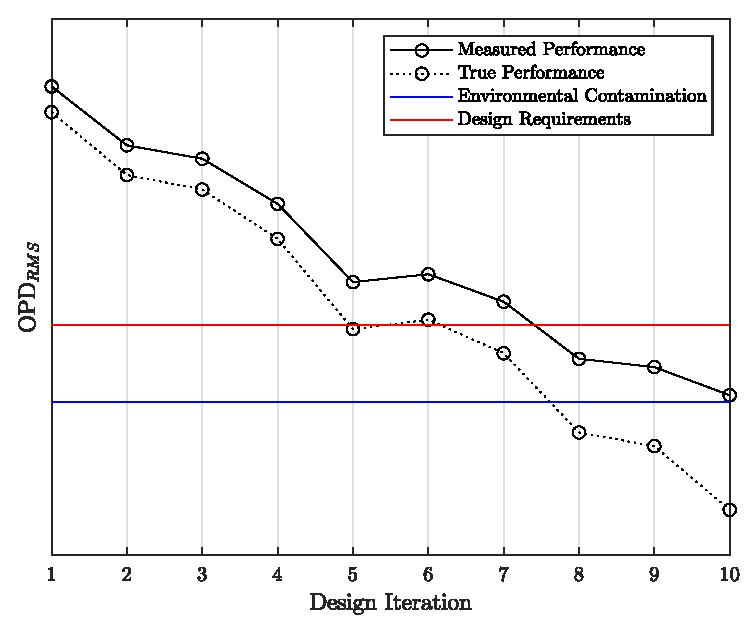
\includegraphics{../matlab/01_introduction/design_iteration.eps}
  \caption{Hypothetical iterative design process of an airborne directed-energy system.  The required performance level is shown by the red line and the testing environment's contamination is shown by the blue line.}
  \label{fig:01_design_iteration}
\end{figure}
This process seeks to obtain a design that meets a required level of performance shown in red.
If only the measured data is used to assess the system's performance three additional iterative changes are needed to achieve a usable design which can add significantly to the development time and costs.
If the environmental contamination is greater than the design requirement, the measured performance will never reach the required performance criteria.
When the true performance of a system is significantly higher than the environmental contamination, the measured performance is not significantly greater than the true performance.
The measured performance becomes significantly greater that the true performance when the true performance is less than the environmental contamination.

This dissertation will primary examine the environmental contamination due to acoustic noise within the wind tunnel.
In Chapter \ref{chap:03_optical_acoustics} it will look at the optical disturbances caused by acoustic waves from some simple plane and spherical waves to a process for estimating the acoustic environment within the test section of a wind tunnel.
The strength of an spherical acoustic wave will be assessed with both microphone and optical measurements.
Multi-dimensional spectral techniques will be used to analyze optical wavefronts in Chapter \ref{chap:04_dispersion} and filter optical wavefronts in Chapter \ref{chap:06_single_filter}.
These filtering techniques will contain some optical contamination particularly in regions where the various signal components interfere with one another.
In order to further reduce the optical contamination, Chapter \ref{chap:07_multiple_filter} will utilize additional sensor information from both microphones and accelerators to remove some of the overlapping contamination to obtain a better picture of the actual optical performance of an airborne directed-energy system from ground test measurements.

% !TEX root = catron-dissertation.tex
\epstopdfsetup{outdir=./images/02_background/}

\chapter{Literature Review}
\label{chap:02_lit_review}
The literature review will consist of primarily two sections.
The first section will examine aero-optics while the second will look at acoustics inside of ducts.
\section{Aero-Optics}
Optical communication and directed energy systems require a tightly focused beam on target in order to meet system performance objectives.
The farfield performance of airborne optical systems can be degraded by the nearfield flow that becomes optically active at compressible flow speeds.
``Aero-optics'' is the study of the optical effect of these nearfield flow disturbances.
Examples of important aero-optical flows that have been studied extensively include boundary layers \cite{Gordeyev-2014-jcJndkHM,Smith-2013-VXArwwux,Wang-2012-gJ7rttg7}, shear layers \cite{Fitzgerald-2004-DgAgbreK,Rennie-2008-Wku6NheG}, shock waves \cite{Jumper-2013-8KtN3pue}, and even tip vortices \cite{Porter-2013-pQcNWHJ6}.
The effect of acoustic disturbances on aero-optical measurements has also been shown in both flight testing \cite{DeLucca-2018-gBQdjTmT} and ground testing \cite{Catron-2018-DdVp6VZf,Catron-2020-x8njYmmu}.

In these optically active flows the index-of-refraction, $n$, varies locally as does the other fluid properties.
Gladstone and Dale \cite{Gladstone-1863-ND4wtDT9} found that the index-of-refraction is primarily a function of density with a loose dependence on the wavelength of light.
Gladstone and Dale proposed a ``specific refractive energy'' now known as the Gladstone-Dale constant, $K_{GD}$,
\begin{equation}
  K_{GD} = \frac{n-1}{\rho}\textrm{.}
  \label{eqn:02_gladstone_dale_constant}
\end{equation}
For air the refractive index can be related to state quantities \cite{Valley-1965-F3k3cmv6}
\begin{equation}
  n-1 = 77.6\times 10^{-6}\frac{P}{T}\left(1+\frac{7.53\times10^{-3}}{\lambda^2}\right)\textrm{,}
  \label{eqn:02_refractive_index_ptlambda}
\end{equation}
where $P$ is in mbar, $T$ is in K, and $\lambda$ is in $\mu$m.
By combining this relationship with the ideal gas law, the Gladstone-Dale constant can be determined as a function of light wavelength,
\begin{equation}
  K_{GD} = 2.23\times10^{-4}\left(1+\frac{7.53\times10^{-3}}{\lambda_{\mu m}^2}\right) \: \left[\frac{m^3}{kg}\right]\textrm{.}
  \label{eqn:02_gladstone_dale_wavelength}
\end{equation}
The Gladstone-Dale constant for air over the visible range is shown in Figure \ref{fig:02_gladstone_dale_wavelength}.
\begin{figure}
  \centering
  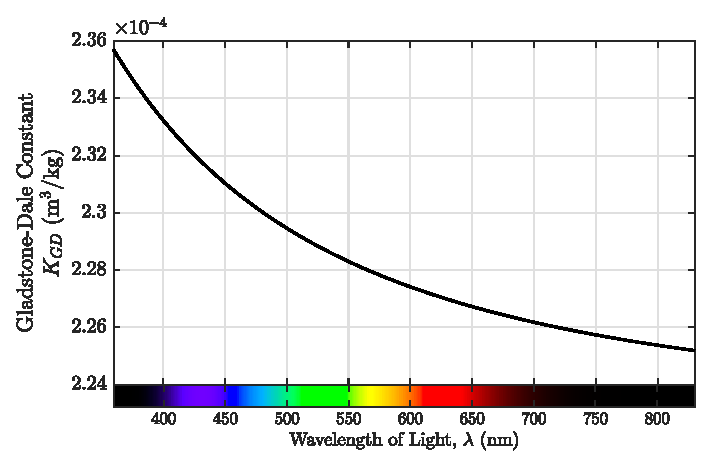
\includegraphics{../matlab/02_background/gladstone_dale_wavelength.eps}
  \caption{Gladstone-Dale constant for air over the visible wavelength range.}
  \label{fig:02_gladstone_dale_wavelength}
\end{figure}
While the value for $K_{GD}$ does vary over the visible range, it is only a few percent, and many sources use an average value of 2.27$\times10^{-4}$ m$^3$/kg for the visible and near-infrared \cite{Gardiner-1980-reW8xrCb}.
The Gladstone-Dale relationship is typically presented as
\begin{equation}
  n = 1+K_{GD}\rho
  \label{eqn:02_gladstone_dale_relation}
\end{equation}
but when applied to situations where there are significant fluctuations in the flow an alternate form is often more useful
\begin{equation}
  n'=K_{GD}\rho'
  \label{eqn:02_gladstone_dale_relation_fluctuating}
\end{equation}
where $'$ denotes the quantity represents the fluctuating component ($n' = n-\bar{n}$).

When a beam with an initially planar wave front passes through a region of optical active flow its wave front aberrated
The optical path length ($\opl$) at any point in the beam can be obtained by integrating the index of refraction along the propagation of an optical ray \cite{Klein-1986-8Vx29RfE}.
\begin{equation}
  \opl (x,y,t) = \int^{s_2}_{s_1} n(x,y,z,t)ds
  \label{eqn:02_opl}
\end{equation}
The optical path difference ($\opd$), is then the spatially-averaged $\textrm{OPL}$ over an aperture removed from the OPL.
\begin{equation}
  \opd(x,y,t) = \opl(x,y,t)-\langle\opl(x,y,t)\rangle
  \label{eqn:02_opd}
\end{equation}
When working with fluctuating components, the $\opd$ can be calculated directly
\begin{equation}
  \opd(x,y,t) = \int^{s_2}_{s_1} n'(x,y,z,t)ds \textrm{.}
  \label{eqn:02_opd_n}
\end{equation}

When $\opd$ is combined with the beam intensity profile, one can compute the farfield complex amplitude distribution using the Fraunhofer approximation \cite{Goodman-1968-zPUmuuzx}.
\begin{equation}
  U(x_0,y_0,t)\propto\iint_{Ap}\exp\left\{\frac{2\pi j}{\lambda}\left[\opd(x_1,y_1,t)-\frac{(x_0x_1+y_0y_1)}{z}\right]\right\}dx_1dy_1
  \label{eqn:02_fraunhofer}
\end{equation}
where $U$ is the complex amplitude, the subscripts 0 and 1 represent the coordinates of the farfield and nearfield respectively.
The intensity can be computed from the complex amplitude via: $I = UU^\ast$.
For cases in which optical aberrations are nonexistent (i.e. $\opd(x,y,t)=0$), the farfield irradiance pattern that results from Equation \ref{eqn:02_fraunhofer} is caused entirely by diffraction from the optical aperture, and is referred to as the “diffraction-limited” irradiance pattern.
For a beam with a flat wave front and circular aperture, the farfield irradiance pattern is the Airy’s disk, and the peak irradiance at the center of the disk, $I_0$ , is the maximum irradiance that can be achieved by the optical system:
\begin{equation}
  I_0 = \left(\frac{kAp^2}{8z}\right)^2
  \label{eqn:02_airy_pattern}
\end{equation}
where $k$ is the wavenumber ($k=2\pi /\lambda$), $Ap$ is the aperture diameter, and $z$ is the distance from the aperture.
In the presence of aero-optical aberrations, $\opd(x,y,t)$ is non-zero, and the farfield irradiance pattern in this case tends to be more spread out and diffuse than the diffraction-limited case; furthermore, the beam may be shifted off target by optical tip/tilt imposed by the aberrations.

The Strehl ratio ($\sr$), is the ratio of intensity on target ($I$) to the diffraction-limited on target intensity ($I_0$):
\begin{equation}
  \sr=\frac{I}{I_0}
  \label{eqn:02_strehl_simple}
\end{equation}
The Strehl ratio can be computed accurately by applying Equation \ref{eqn:02_fraunhofer} twice, once for the diffraction-limited case to obtain $I_0$, and a second time with the $\opd$ field due to aero-optical aberrations included to obtain $I$.
The farfield performance, can also be estimated via the Mar\'{e}chal approximation:
\begin{equation}
  \sr(t) \equiv \frac{I(t)}{I_0} \approx \exp \left\{-\left[\frac{2\pi \opdrms(t)}{\lambda}\right]^2\right\}
  \label{eqn:02_strehl_ratio}
\end{equation}
where $\opdrms$ is the spatial rms of the wave front and $\lambda$ is the wavelength of the beam.
\begin{figure}
  \centering
  \begin{subfigure}[t]{0.45\textwidth}
    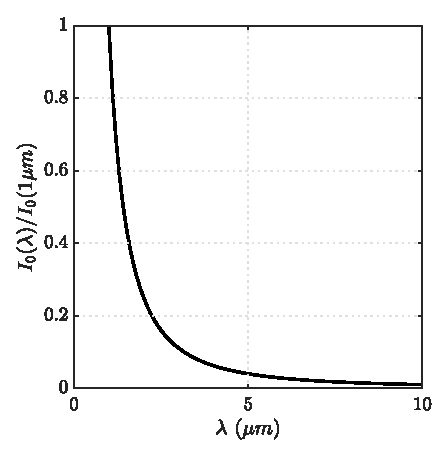
\includegraphics{../matlab/02_background/farfield_intensity.eps}
    \caption{}\label{fig:02_farfield_intensity}
  \end{subfigure}
  ~
  \begin{subfigure}[t]{0.45\textwidth}
    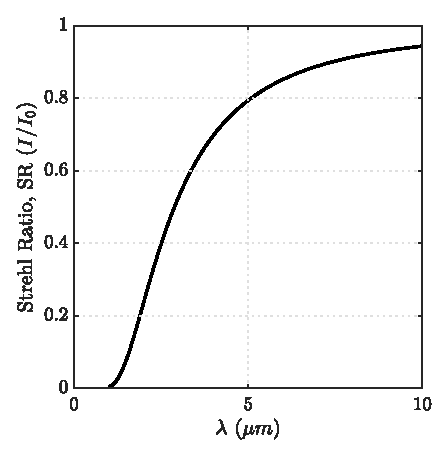
\includegraphics{../matlab/02_background/all_strehl_ratio.eps}
    \caption{}\label{fig:02_all_strehl_ratio}
  \end{subfigure}
  \caption{(\subref{fig:02_farfield_intensity}) Diffraction limited on target intensity as a function of wavelength normalized by the value at $\lambda$ = 1 $\mu$ m. (\subref{fig:02_all_strehl_ratio}) Strehl ratio as a function of wavelength for an aberration that gives SR = 0.95 at $\lambda$ = 10.6 $\mu$m.}
  % \label{FIG:airy_strehl}
\end{figure}
Equation \ref{eqn:02_strehl_ratio} shows a key relationship between $\opd$, wavelength, and the farfield performance, plotted in Figure \ref{fig:02_all_strehl_ratio}.
On the other hand, Equation \ref{eqn:02_airy_pattern} shows that the diffraction-limited farfield irradiance increases as the wavelength is shortened, plotted in Figure \ref{fig:02_farfield_intensity}.
Together, Figure \ref{fig:02_farfield_intensity} and \ref{fig:02_all_strehl_ratio} show that as modern optical systems move to shorter wavelengths to increase $I_0$, aero-optical aberrations cause a much more serious degradation of the Strehl ratio, illustrating why aero-optical considerations are critical in the development of any airborne optical system.

Figure \ref{fig:02_necessary_opd} shows the $\opdrms$ necessary to achieve various Strehl ratios over a range of wavelengths.
\begin{figure}
  \centering
  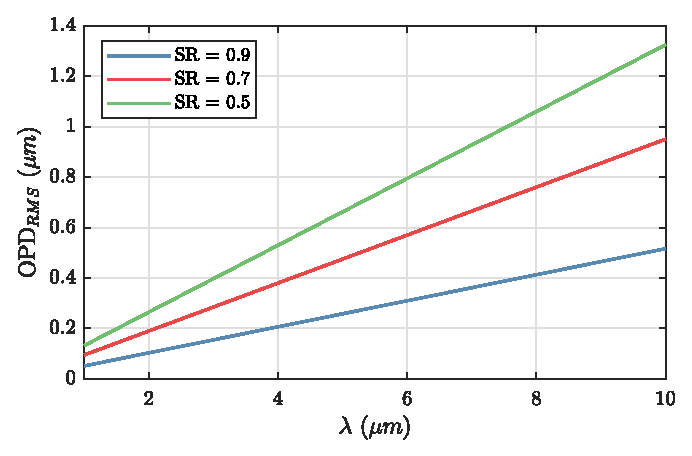
\includegraphics{../matlab/02_background/necessary_opd.eps}
  \caption{$\opdrms$ values necessary to obtain Strehl ratios of 0.9, 0.7, and 0.5 over a range of wavelengths.}
  \label{fig:02_necessary_opd}
\end{figure}
As the wavelength of light decreases the required $\opdrms$ decreases linearly for a fixed Strehl ratio.


\subsection{Typical Optical Wavefront Measurement System}





\begin{figure}
  \centering
  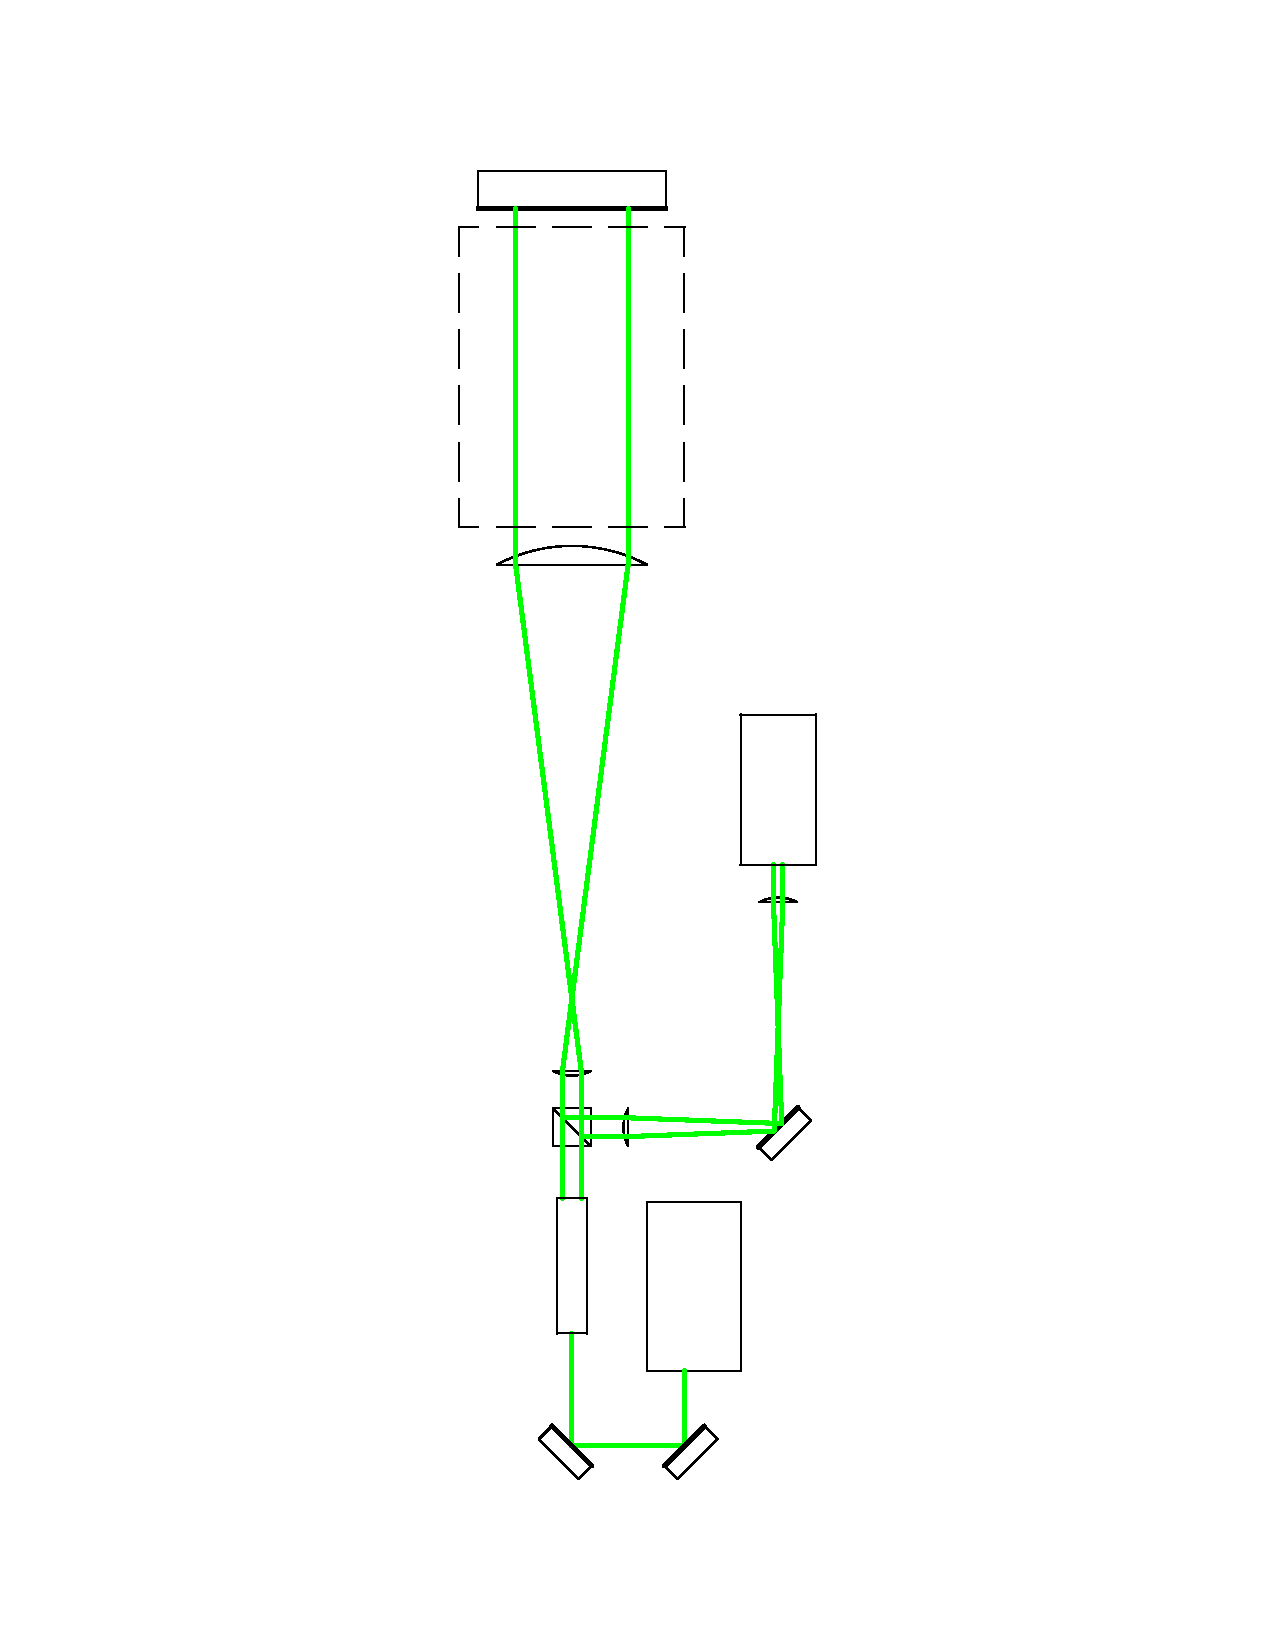
\includegraphics[width=2.5in,clip,trim=200 75 200 75]{../cad/wavefront_setup.pdf}
  \put(-72,62){\rotatebox{90}{\Large LASER}}
  \put(-145,78){\rotatebox{90}{BEAM}}
  \put(-135,65){\rotatebox{90}{EXPANDER}}
  \put(-150,200){\rotatebox{90}{\Large PRIMARY TELESCOPE}}
  \put(-130,400){\rotatebox{90}{\Large MEASUREMENT}}
  \put(-112,427){\rotatebox{90}{\Large REGION}}
  \put(-95,160){\rotatebox{60}{\Large REIMAGING}}
  \put(-80,155){\rotatebox{60}{\Large TELESCOPE}}
  \put(-10,245){\rotatebox{90}{\Large WAVEFRONT}}
  \put(5,260){\rotatebox{90}{\Large SENSOR}}
  \caption{Typical double-pass optical wavefront measurement setup.}
  \label{fig:02_typical_wavefront_system}
\end{figure}




\subsection{A Brief History of Aero-Optics}
The field of aero-optics began with an investigation by Liepmann \cite{Liepmann-1952-89GQ7wyA} into the limits of sensitivity of schlieren systems when used in high-speed flow analysis.
Liepmann used geometric optics to analyze a small-diameter beam and derive its mean-squared fluctuating deflection angle, $\left<\theta^2\right>$.
Liepmann propagated the beam in the $y$ direction and assumed the index of refraction changes in the $x-z$ plane were statistically similar.
Liepmann's analysis for a boundary layer of thickness $\delta$ resulted in
\begin{equation}
  \left<\theta^2\right> = \frac{1}{[n_0(\delta)]^2}\int_0^\delta\int_0^\delta n_0(y)n_0(\zeta)\left<\left(\frac{\partial\nu}{\partial y}\right)^2\right>R_v(|y-\zeta|)dyd\zeta
  \label{eqn:02_liepmann_deflection_angle}
\end{equation}
where the index of refraction is determined from $n=n_0(y)(1+\nu)$ and $R_v(|y-\zeta|)$ is the correlation function for the index variation.
This analysis introduced the concept of a linking equation that allows one to predict time-averaged optical degradation to turbulent flow statistical measurements.

\section{Acoustics}

\subsection{Basic Acoustics}


Starting with the conservation of mass,
\begin{equation}
  \frac{\partial\rho}{\partial t}+\nabla\cdot\left(\rho\mathbf{u}\right)=0  \textrm{,}
  \label{eqn:02_cons_of_mass}
\end{equation}
and separating the density into a time-averaged ($\rho_0$) and fluctuating portion ($\rho'$), $\rho = \rho_0+\rho'$.
The fluctuating conservation of mass equation is obtained by separating the density ($\rho = \rho_0+\rho'$) into a temporally averaged density, $\rho_0$, and a

\begin{equation}
  \frac{\mathbf{D}\rho'}{\mathbf{Dt}}+\nabla\cdot\left(\rho_0\mathbf{u}\right)=0
  \label{eqn:02_cons_of_mass_fluc}
\end{equation}





For acoustics waves of frequency less than $10^9$ Hz the compression of the fluid can be assumed to be adiabatic \cite{Morse-1968-yygEdQZf}.


\begin{equation}
  \left.\frac{\partial p}{\partial\rho}\right|_s = c_0^2
  \label{eqn:02_speed_of_sound}
\end{equation}

\subsection{Duct Acoustics}
Acoustic waves are often enclosed inside of somesort of structure.
This section will look at acoustics when confined to a duct in which the acoustic waves primarily travel along one-axis and have walls confining the acoustics along the other two axes as is the case inside of a wind tunnel.
Figure \ref{fig:02_duct_drawing} shows the diagram used for deriving the acoustic properties inside of a constant area duct.
\begin{figure}
\centering
  % \fbox{
    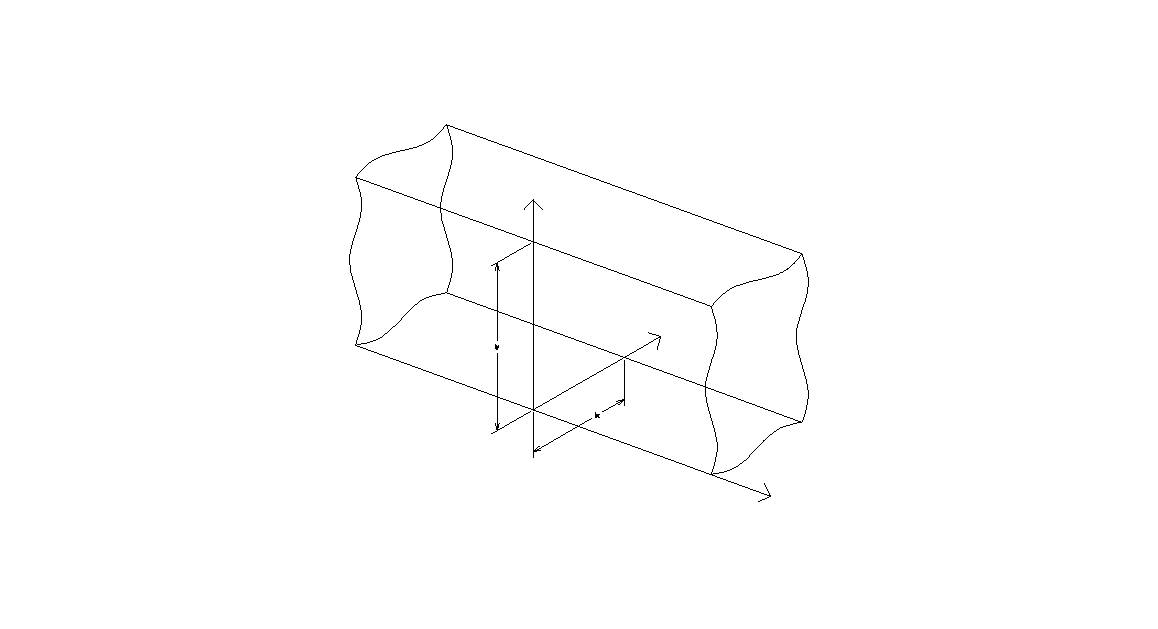
\includegraphics[trim=2.2in 0.7in 2.2in 0.7in,clip,width=4.5in]{../autocad/02_background/duct_drawing.eps}
    \put(-155,62){\fcolorbox{white}{white}{$l_x$}}
    \put(-227,113){\fcolorbox{white}{white}{$l_y$}}
    \put(-103,119){$\mathbf{x}$}
    \put(-198,220){$\mathbf{y}$}
    \put(-26,4){$\mathbf{z}$}
  % }
  \caption{Duct with a rectangular cross-section.}
  \label{fig:02_duct_drawing}
\end{figure}

This derivation is primarily influenced from Munjal \cite{Munjal-2014-w28y4EyP} along with Jacobsen and Juhl \cite{Jacobsen-2013-PHD3v3YZ}.
The primary assumption used in this derivation is that the duct is of constant cross-section.
This means that all mean quantities ($\rho_0$, $\mathbf{u_0}$, ...) a constant throughout space and time.
Starting with the linearized inviscid forms of the conservation of mass,
\begin{equation}
  \frac{\mathbf{D}\rho}{\mathbf{Dt}} + \rho_0\nabla\cdot\mathbf{u} = 0 \textrm{,}
  % \frac{\partial\rho}{\partial t} + \mathbf{u}\cdot\nabla\rho + \rho_0(\nabla\cdot\mathbf{u}) = 0 \textrm{,}
  \label{eqn:02_cons_mass}
\end{equation}
and conservation of momentum,
\begin{equation}
  \rho_0\frac{\mathbf{Du}}{\mathbf{Dt}} + \nabla p = 0 \textrm{.}
  % \rho_0\frac{\partial\mathbf{u}}{\partial t} + \rho_0(\mathbf{u_0}\cdot\nabla)\mathbf{u} + \nabla p = 0 \textrm{.}
  \label{eqn:02_cons_mom}
\end{equation}
The definition of the speed of sound (Equation \ref{eqn:02_speed_of_sound}) is then substituted into Equation \ref{eqn:02_cons_mass},
\begin{equation}
  \frac{1}{c_0^2}\frac{\mathbf{D}p}{\mathbf{Dt}} + \rho_0\nabla\cdot\mathbf{u} = 0 \textrm{,}
  % \frac{1}{c_0^2}\frac{\partial p}{\partial t} + \frac{1}{c_0^2}(\mathbf{u}\cdot\nabla p) + \rho_0(\nabla\cdot\mathbf{u}) = 0 \textrm{,}
  \label{eqn:02_cons_mass_p}
\end{equation}
where $c_0$ is the speed of sound at average fluid properties ($\rho_0$, $p_0$, $T_0$, ...).
Next the difference between the material derivative ($\mathbf{D}/\mathbf{Dt}$) of Equation \ref{eqn:02_cons_mass_p} and the partial derivative ($\partial/\partial\mathbf{x}$) of Equation \ref{eqn:02_cons_mom} with respect to space is taken which results in the convected 3-D wave equation,
\begin{equation}
  \left(\frac{\mathbf{D}^2}{\mathbf{Dt}^2}-c_0^2\nabla^2\right)p=0\textrm{.}
  \label{eqn:02_wave_conv_3_c}
\end{equation}
Expanding the material derivative and dividing by $c_0^2$,
\begin{equation}
  \left(\frac{1}{c_0^2}\frac{\partial^2}{\partial t^2} + \frac{2\mathbf{M}}{c_0}\frac{\partial^2}{\partial t\partial\mathbf{x}} - (1-\mathbf{M}^2)\nabla^2\right)p = 0 \textrm{,}
  \label{eqn:02_wave_conv_expand}
\end{equation}
where $\mathbf{M} = \mathbf{u_0}/c_0$.
By using the fact that $c_0=\omega/k_0$, Equation \ref{eqn:02_wave_conv_3_c} can be written in a more convent form,
\begin{equation}
  \left(\frac{1}{\omega^2}\frac{\partial^2}{\partial t^2} + \frac{2\mathbf{M}}{\omega k_0}\frac{\partial^2}{\partial t\partial\mathbf{x}} - \frac{1-\mathbf{M}^2}{k_0^2}\nabla^2\right)p = 0 \textrm{,}
  \label{eqn:02_wave_conv_3}
\end{equation}
where $\omega$ is the angular frequency and $k_0$ is the total wavenumber.

At this point the pressure field is going to written in a complex form and assumed to be separable in both time and space such that $\hat{p}(\mathbf{x},t) = \hat{p}(x,y)\hat{p}(z)\hat{p}(t)$.
The temporal solution is assumed to take the form
\begin{equation}
  \hat{p}(t) = \exp\left\{j\omega t\right\} \textrm{.}
  \label{eqn:02_pressure_solution_time}
\end{equation}
This results in the spatial component of the convecting wave equation
\begin{equation}
  \left((1-\mathbf{M}^2)\nabla^2-2jk_0\mathbf{M}\nabla+k_0^2\right)\hat{p}(x,y)\hat{p}(z) = 0 \textrm{.}
  \label{eqn:02_wave_conv_space}
\end{equation}
This can be further split into axial and cross-sectional components by splitting $k_0$ into components,
\begin{equation}
  k_0 = \sqrt{k_{xy}^2+k_z^2} \textrm{,}
  \label{eqn:02_k0}
\end{equation}
and because the mean flow is only in the axial direction ($\mathbf{M} = M\mathbf{\hat{k}}$).
The cross-sectional component is a typical Helmholtz equation
\begin{equation}
  \left(\frac{\partial^2}{\partial x^2}+\frac{\partial^2}{\partial y^2}\right)\hat{p}_{xy}(x,y)+k_{xy}^2\hat{p}(x,y) = 0 \textrm{,}
  \label{eqn:02_wave_xy}
\end{equation}
whos solution,
\begin{equation}
  \hat{p}(x,y) = \Psi_m(x,y) \textrm{,}
  \label{eqn:02_pressure_solution_xy}
\end{equation}
is one of infinity many eigen-function solutions with discrete wavenumbers, $k_m$.
The axial component of the convecting wave equation,
\begin{equation}
  (1-M^2)\frac{\partial^2\hat{p}(z)}{\partial z^2} - 2jk_0M\frac{\partial\hat{p}(z)}{\partial z} + k_z^2\hat{p}(z) = 0 \textrm{,}
  \label{eqn:02_wave_z}
\end{equation}
retains the total wavenumber in second term which means its solution will depend on the cross-sectional wavenumber value at cross-sectional mode.
The solution to the axial convecting wave equation,
\begin{equation}
  \hat{p}(z) = p^+_m\exp{\left\{-jk^+_{zm}z\right\}}+p^-_m\exp{\left\{+jk^-_{zm}z\right\}} \textrm{,}
  \label{eqn:02_pressure_solution_z}
\end{equation}
has waves traveling in both directions with the axial wavenumber in each direction for a given mode
\begin{equation}
  k^\pm_{zm} = \frac{\mp Mk_0+\sqrt{k_0^2-(1-M^2)k_m^2}}{1-M^2} \textrm{.}
  \label{eqn:02_kzm}
\end{equation}

The solution for a three-dimensional acoustic wave in a duct with a constant but arbitrary cross-section in complex pressure is the combination of the component solutions presented in Equations \ref{eqn:02_pressure_solution_time}, \ref{eqn:02_pressure_solution_xy}, and \ref{eqn:02_pressure_solution_z},
\begin{equation}
  \hat{p}(x,y,z,t) = \Psi_m(x,y)\left(p^+_m\exp{\left\{-jk^+_{zm}z\right\}}+p^-_m\exp{\left\{+jk^-_{zm}z\right\}}\right)\exp\left\{j\omega t\right\} \textrm{.}
  \label{eqn:02_pressure_solution_duct}
\end{equation}
The two solutions for a plane wave ($\Psi_m=1$, $k_m=0$) traveling in a duct have a characteristic speed of $u\pm c_0$.
Acoustic modes will travel indefinitly if $k_0^2-(1-M^2)k_m^2>0$ (the quantity inside of the square-root of Equation \ref{eqn:02_kzm}).
This presents a frequency at which a given mode will cut-on,
\begin{equation}
  f_{cuton} = \frac{c_0}{2\pi}\sqrt{(1-M^2)k_m^2} \textrm{.}
  \label{eqn:02_cuton_freq}
\end{equation}
Below this frequency, an acoustic mode will be exponentially attenuated as it travels throught the duct.

\subsubsection{Characteristic Equations of Cross-Sections}
In order to determine the characteristic equations of an acoustic field within a cross-section the solution to Equation \ref{eqn:02_wave_xy} needs to be determined.
A typical boundary condition that is used in the solution of this 2-D Helmholtz equation is using the assumption that the walls are rigid.
\begin{equation}
  \nabla p_{x,y}(x,y)\cdot\mathbf{n}_{wall} = 0
  \label{eqn:02_bc_rigig_wall}
\end{equation}
This boundary condition results in the acoustic waves being perfectly reflected off of the duct walls.
There are several known empirical solution sets of the characteristic equations for specific geometry with the rigid wall assumption.

The first of these solutions is for a rectangular cross-section,
\begin{equation}
  \Psi_{m,n}(x,y) = \cos(k_xx)\cos(k_yy) \textrm{,}
  \label{eqn:02_psi_rect}
\end{equation}
where the wave numbers along each axis are $k_x = m\pi/l_x$ and $k_y = n\pi/l_y$.
The duct has a width of $l_x$ and a height of $l_y$.
The total cross-sectional wave number for use in determining the axial wave numbers is
\begin{equation}
  k_m^2 = k_x^2+k_y^2 \textrm{.}
  \label{eqn:02_wave_number_crosssection}
\end{equation}
Figure \ref{fig:02_cross_section_rect} shows the characteristic functions when m=0:2 and n=0:3 for a rectangular cross-section of width of $l_x$ and height of $l_y$.
\begin{figure}
  \centering
  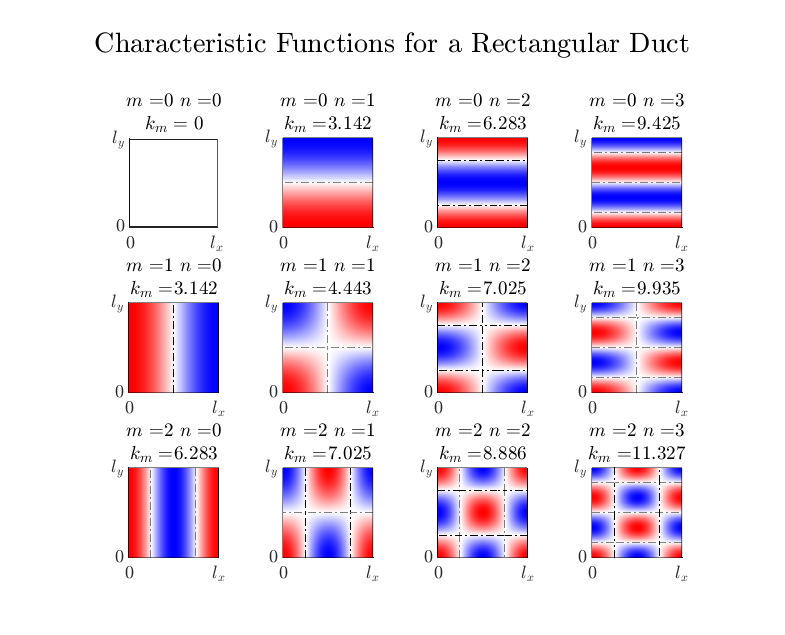
\includegraphics{../matlab/02_background/cross_section_rect.eps}
  \caption{Characteristic solutions to Equation \ref{eqn:02_wave_xy} with rigid wall in a rectangular cross-section where m=0:2 and n=0:3.  Nodal lines are depicted by the dot-dash lines.  The cross-sectional wave numbers, $k_m$, listed are for a duct of unit length and height.}
  \label{fig:02_cross_section_rect}
\end{figure}
The lines depicted in the figure are nodal lines and represent locations where there is zero pressure fluctuations for that acoustic mode.

The second set of known empirical solutions is for a circular cross-section with radius $R$,
\begin{equation}
  \Psi_{m,n}(r,\theta) = J_m(k_{mn}r)\exp\left\{\pm jm\theta\right\} \textrm{,}
  \label{eqn:02_psi_circ}
\end{equation}
where $J_m$ is the $m^\textrm{th}$ Bessel function of the first kind and the $\pm$ indicates the direction of spin.
If the left and right spin coefficients are equal in magnitude then a non-spinning mode is created.
In order to satisfy the solid wall boundary condition $J_m'(k_{mn}R) = 0$ which determines a set of discrete values for the cross-sectional wave number at the $n^\textrm{th}$ zero for the $m^\textrm{th}$ Bessel function.
Figure \ref{fig:02_cross_section_circ} shows the characteristic functions for a circular duct.
\begin{figure}
  \centering
  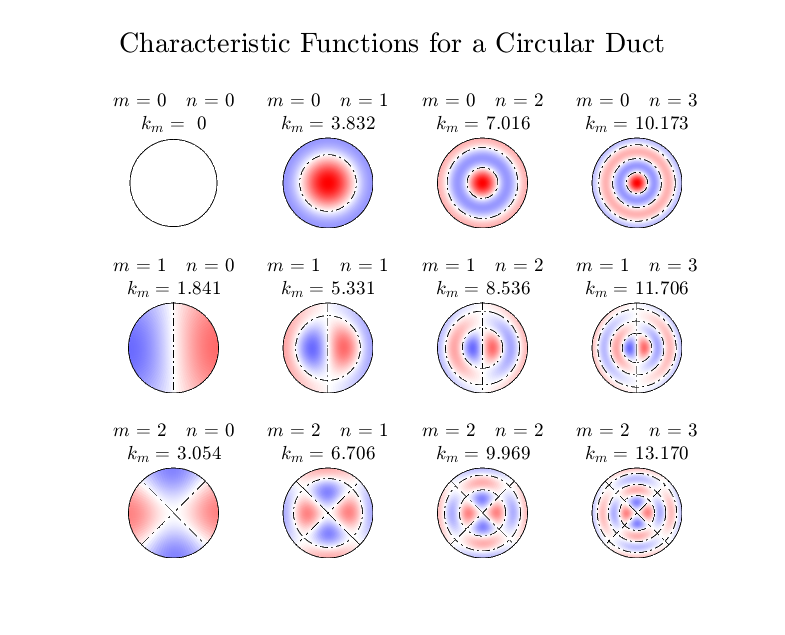
\includegraphics{../matlab/02_background/cross_section_circ.eps}
  \caption{Characteristic solutions to Equation \ref{eqn:02_wave_xy} with rigid wall in a circular cross-section where m=0:2 and n=0:3.  Nodal lines are depicted by the dot-dash lines.  The cross-sectional wave numbers, $k_m$, listed are for a duct of unit radius.}
  \label{fig:02_cross_section_circ}
\end{figure}

% !TEX root = catron-dissertation.tex
\epstopdfsetup{outdir=./images/03_aero_optics_acoustics/}

\chapter{Aero-Optical and Acoustical Coupling}
\label{chap:03}

\begin{itemize}
  \color{red}
  \item Spherical solutions and measurements
  \item Double check microphone and preamp models and settings
  \item Mode marching method
\end{itemize}


Acoustic waves are isentropic compression waves with the fluctuating pressure, $p'$, determining the strength of the wave.
This fluctuating pressure is related to the sound pressure level, $\spl$ by
\begin{equation}
  \spl = 20\log_{10}\left(\frac{p_{rms}}{p_0}\right)
  \label{eqn:03_spl}
\end{equation}
where $p_{rms}$ is the root mean square of the pressure fluctuation, and $p_0$ is the reference pressure (20 $\mu$Pa for air).
The pressure fluctuations can be converted to the density fluctuations via the definition of the speed of sound:
\begin{equation}
  c_0^2 = \left(\frac{\partial p}{\partial \rho}\right)_s=\frac{p'}{\rho'}
  \label{eqn:03_speed_sound}
\end{equation}
where $c_0$ is the speed of sound at mean fluid properties and the subscript $s$ denotes constant entropy.
It can be shown by combining Equations \ref{eqn:02_gladstone_dale_relation_fluctuating} and \ref{eqn:02_opd} that the fluctuating density can be related to the $\opd$,
\begin{equation}
  \opd = K_{GD}\int_{s_1}^{s_2}{\rho'}ds \textrm{.}
  \label{eqn:03_opd_fluct}
\end{equation}
This can be combined with Equation \ref{eqn:03_speed_sound},
\begin{equation}
  \opd = \frac{K_{GD}}{c_0^2}\int_{s_1}^{s_2}{p'}ds \textrm{,}
  \label{eqn:03_opd_pressure}
\end{equation}
to provide a way of computing the optical path difference of a pressure field.

% When the pressure field is known in complex quantities (magnitude and phase), a complex optical path difference can calculated,

% Here the complex pressure field was assumed to be seperable in time and space.
% The measurable $\opd$ is

% This can greatly reduce the computational cost of simulating a beam passing through a pressue or density field that is separable in time and space by only performing the spatial integration once for each temporal frequency component.

\section{Simulating an Optical Wavefront Measurement from an Acoustic Field Function}
\label{chap:03_simulated_beam}
An optical wavefront can be simulated from a complex pressure field by applying Equation \ref{eqn:03_opd_pressure}.
To accomplish this, two separate coordinate systems will need to be defined.
The first is the beam coordinate system, $\mathbf{x}_B $, that will have a measurement aperture, which is typically circular, defined in the xy-plane and propagates in the z-direction.
The second is the acoustic coordinate system, $\mathbf{x}_A$, that will be defined based on the source location or the geometry that the acoustic waves are propagating through.
These to coordinate systems will have a function representing a transform from one to the other
\begin{equation}
  \mathbf{x}_A = R\mathbf{x}_B+T \textrm{,}
  \label{eqn:03_coord_transform}
\end{equation}
where $R$ is a matrix which represents the rotation and $T$ is a vector that represents the translation.

The important parameters for defining the aperture which the beam coordinate system is based are the aperture size, $Ap$, and the number of lenslets or sub-apertures, $N_{lenslets}$.
Assuming that the aperture is either circular or square and the lenslet size and sub-aperture size is approximately $Ap/N_{lenslets}$, the x locations of the center of the sub-apertures go from $-Ap/2(1-1/N_{lenslets})$ to $Ap/2(1-1/N_{lenslets})$ by steps of $Ap/N_{lenslets}$ with the y locations having the same values.
This gives a matrix representing both $x_{Ap}$ and $y_{Ap}$ that is $N_{lenslets}$ by $N_{lenslets}$.
For the purpose of removing piston, tip, and tilt and creating a mask that represents the beam aperture, the radial coordinates, $\rho_{Ap}$ and $\theta_{Ap}$, of the aperture should also be calculated.
A circular beam will have a mask defined by,
\begin{equation}
  Mask_{Ap} =
  \begin{cases}
    1, & \text{if } \rho_{Ap}\leq Ap/2 \\
    0, & \text{otherwise.}
  \end{cases}
\end{equation}
The beam coordinate frame is the aperture coordinates extruded in the z-direction over the range of desired z-values.

After the beam coordinates are transformed into the acoustic coordinates using Equation \ref{eqn:03_coord_transform}, the complex pressure field, $\hat{p}(x,y,z,t)$ can be calculated at the points that are within the optical beam.
If the pressure field is separable into spatial and temporal components, than the integration along the beam length only needs to be done once for each temporal frequency,
\begin{equation}
  \widehat{\opd}(x,y) = \frac{K_{GD}}{c_0^2}\int_{z_1}^{z_2} \hat{p}(x,y,z)_{Ap}dz \textrm{,}
  \label{eqn:03_opd_complex}
\end{equation}
where $\widehat{\opd}(x,y)$ is the complex optical path difference as measured in the aperture plane.
If a complex density field is known instead, than Equation \ref{eqn:03_opd_complex} becomes
\begin{equation}
  \widehat{\opd}(x,y) = K_{GD}\int_{z_1}^{z_2} \hat{\rho}(x,y,z)_{Ap}dz \textrm{.}
  \label{eqn:03_opd_complex_density}
\end{equation}
For the purposes of calculating temporally mean optical properties of simulated beam passing through a known complex pressure or density field a phase vector was defined,  $\phi = [0, 2\pi)$.
The measurable component as a function of phase is
\begin{equation}
  \opd(x,y,\phi) = \real\left[\widehat{\opd}(x,y)\exp\{-j\phi\}\right] \textrm{,}
  \label{eqn:03_opd_real_phase}
\end{equation}
or as a function of time for all temporal frequencies,
\begin{equation}
  \opd(x,y,t) = \real\left[\sum\widehat{\opd}(x,y)\exp\{-j\omega t\}\right] \textrm{,}
  \label{eqn:03_opd_real}
\end{equation}
where there is a separate $\widehat{\opd}(x,y)$ computed for each temporal frequency.
One of the more important measurements that can be calculated from $\opd$ is the spatial RMS, $\opdrms$, which is calculated at each time or phase step at the points where the aperture mask equals one.

\section{Simple Examples of Acoustic-Optical Coupling}
Two basic acoustic pressure fields will be numerically examined for their optical properties.
The first will be a planar acoustic wave that will be numerically simulated over a variety of conditions.
The second will be a spherical acoustic wave that will be both numerically simulated and validated experimentally.

\subsection{Planar Acoustic Waves}
A planar wave is the simplest solution to the wave equation and varies only in time and the direction of travel.
A planar wave can be calculated from the set of solutions for duct acoustics, Equation \ref{eqn:02_pressure_solution_duct}, given that $\Psi_m(x,y)=1$,
\begin{equation}
  \hat{p}(z,t) = p_m\exp\left\{j(\omega t \mp k_{zm}^\pm z)\right\} \textrm{.}
  \label{eqn:03_plane_wave}
\end{equation}
This section will show several plots to show the effect that acoustic waves have on the optical wavefront of a planar wave with the general geometry shown in Figure \ref{fig:03_planar_sample_domain}.
\begin{figure}
  \centering
  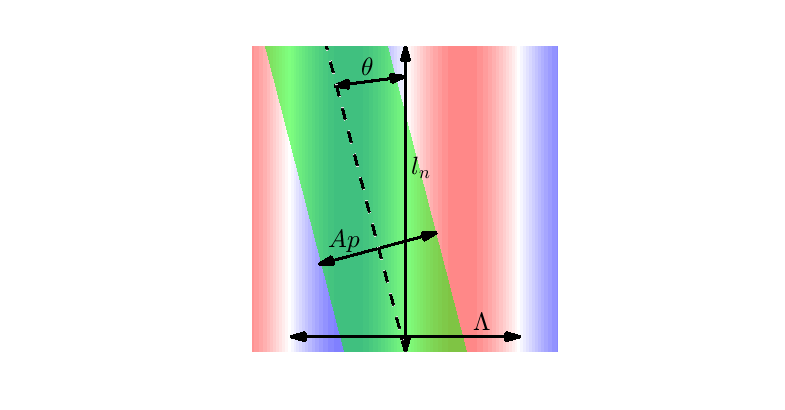
\includegraphics{../matlab/03_aero_optics_acoustics/planar_sample_domain.eps}
  \caption{General geometry for various sample calculations for showing the acoustic-optical coupling effect.}
  \label{fig:03_planar_sample_domain}
\end{figure}
For the following example, $l_n$ is the width of the acoustic disturbance (for example, the width of the wind tunnel), $\theta$ is the angle between the planar acoustic wave and the beam direction, $A_p$ is the aperture diameter of the beam, and $\Lambda$ is the wavelength of the acoustic wave.

Figure \ref{fig:03_planar_sample_calc_3} shows the time averaged $\opdrms$ per meter of beam propagation when the beam path is parallel ($\theta=0$) to the peaks and troughs of the planar acoustic wave as $\spl$ is varied.
\begin{figure}
  \centering
  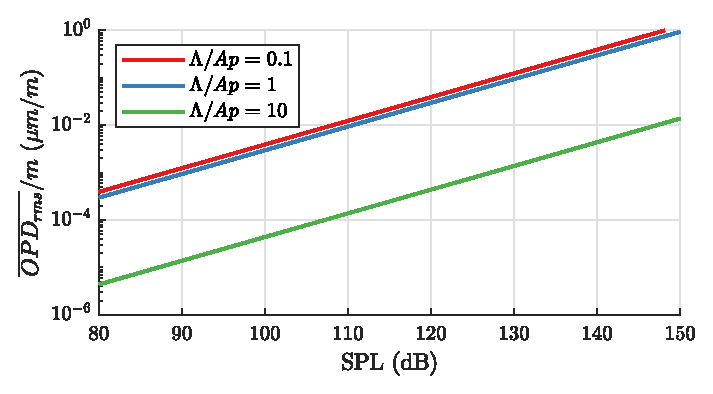
\includegraphics{../matlab/03_aero_optics_acoustics/planar_sample_calc_3.eps}
  \caption{Theoretical time-averaged $\opdrms$ per meter of beam propagation as a function of sound pressure level, $\spl$, for several $\Lambda/Ap$ ratios and $\theta=0$.}
  \label{fig:03_planar_sample_calc_3}
\end{figure}
As the sound pressure level increases the time averaged $\opdrms$ also increases and can easily reach the point of being a significant factor in the measured optical disturbance.
There is little difference between 0.1 and 1 $\Lambda/Ap$, but as the wavelength gets much larger compared to the beam diameter, then the optical effect of the noise is greatly reduced, this effect is known as aperture filtering \cite{Siegenthaler-2005-KQ2HGmfp}.

Aperture filtering is more clearly shown in Figure \ref{fig:03_planar_sample_calc_1}.
\begin{figure}
  \centering
  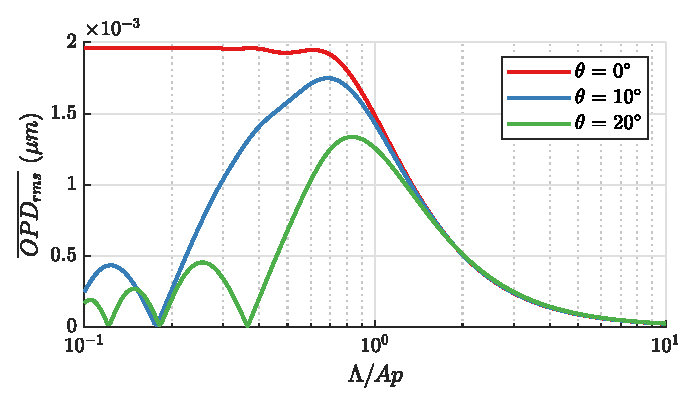
\includegraphics{../matlab/03_aero_optics_acoustics/planar_sample_calc_1.eps}
  \caption{Theoretical time-averaged $\opdrms$ for a rms sound pressure of 1 Pa ($\spl$ of 94 dB), $l_n$ of 1 m, and various angles and $\Lambda/Ap$ ratios.}
  \label{fig:03_planar_sample_calc_1}
\end{figure}
As the $\Lambda/Ap$ ratio increases from 0.1, time-averaged $\opdrms$ remains fairly constant until it starts to drop around $\Lambda/Ap$ of 0.7 and starts to asymptotically approach zero which it basically reaches by $\Lambda/Ap$ of 10.
Figure \ref{fig:03_planar_sample_calc_1} also shows the effect of changing the beam angle, $\theta$, through the acoustic field.
For nonzero $\theta$, the beam encounters alternating high and low index of refraction as it passes through the test region, so that the time-averaged $\opdrms$ begins to decrease compared to the $\theta = 0^\circ$ case below $\Lambda/Ap=1$.
There are also points of zero optical disturbance that occur at $\theta_{zero}=\tan^{-1}(n\Lambda/l_n)$ for $n\neq0$; these points occur because the peaks and valleys of the optical disturbance caused by the sound wave effectively cancel out over the length of the integration path, $l_n/\cos\theta$.

Figures \ref{fig:03_planar_sample_calc_3} and \ref{fig:03_planar_sample_calc_1} show the optical effect of plane acoustic waves in a no-flow environment.
The effect of wind-tunnel flow is to stretch (downstream-traveling waves) or compress (upstream-traveling waves) the wavelength of the acoustic noise thereby altering the filtering effect of the beam aperture.
Figure \ref{fig:03_planar_sample_calc_2} shows a typical optical disturbance from the two transverse acoustic waves (u+c and u-c) present in a wind tunnel at Mach 0.6.
\begin{figure}
  \centering
  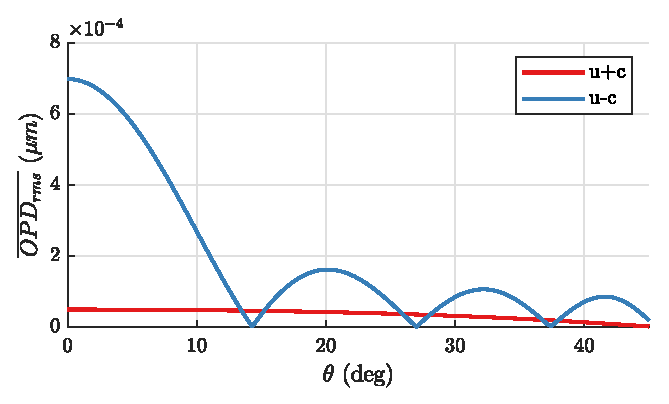
\includegraphics{../matlab/03_aero_optics_acoustics/planar_sample_calc_2.eps}
  \caption{Theoretical time-averaged $\opdrms$ for the two acoustic waves (u+c and u-c) for the blade pass frequency (534 Hz) at Mach 0.6 with a RMS sound pressure of 1 Pa ($\spl$ of 94 dB), $l_n$ of 1 m, and $Ap$ of 15 cm.}
  \label{fig:03_planar_sample_calc_2}
\end{figure}
Both waves have a RMS sound pressure of 1 Pa and the beam has an aperture of 15 cm and propagates through a 1 m acoustic field inside the tunnel.
Over a vast majority of the look back angles the upstream-traveling acoustic wave has a much greater effect on the optical disturbance compared to the downstream-traveling acoustic wave, due to the much shorter wavelength of the upstream-traveling waves which is less affected by aperture filtering.
However, the upstream-traveling wave goes through several zero points so the downstream-traveling wave dominates at some look back angles.

% In summary, Figures \ref{fig:03_planar_sample_calc_3} to \ref{fig:03_planar_sample_calc_2} give an example of how planar acoustic waves are expected to affect a beam traveling a finite distance $l_n$ at an angle $\theta$ through the acoustic field.

\subsection{Spherical Acoustic Waves}
The acoustic field from an speaker maybe assumed to be a spherical wave from a pulsating point if the frequency is sufficiently low and measurement region is far enough away from the source \cite{Randall-1951-9NtPPXPq}.
This pressure field when converted to complex pressure is represented by
\begin{equation}
  \hat{p}(r,t) = \frac{A_0}{r}\exp\left\{-j(kr-\omega t)\right\} \textrm{,}
  \label{eqn:03_spherical_pressure}
\end{equation}
where $A_0$ is the fluctuating pressure strength and $r$ is the distance from the source to the measurement point.
The RMS pressure of this field can be represented by
\begin{equation}
  p_{rms} = \frac{|A_0|}{r\sqrt{2}} \textrm{.}
  \label{eqn:03_spherical_pressure_rms}
\end{equation}

\subsubsection{Theoretical OPD Measurements}
A set of optical properties where calculated for a beam passing through a spherical acoustic field as defined by a point source using the process discribed previously in Chapter \ref{chap:03_simulated_beam}.
These calculations used an circular aperture size of 0.25-m in diameter consisting of 32x32 sub-apertures, an acoustic wavelength, $\Lambda$, of $Ap/4$ to $10Ap$, and a distance from the point source to the center of the aperture, $R$, of $5Ap$ to $25Ap$.
The beam was integrated over $\pm5$-m from the plane of the point source with 25 phase step used to calculate mean values.

The result of these simulated acoustic fields is shown in Figure \ref{fig:03_spherical_sample}.
\begin{figure}
  \centering
  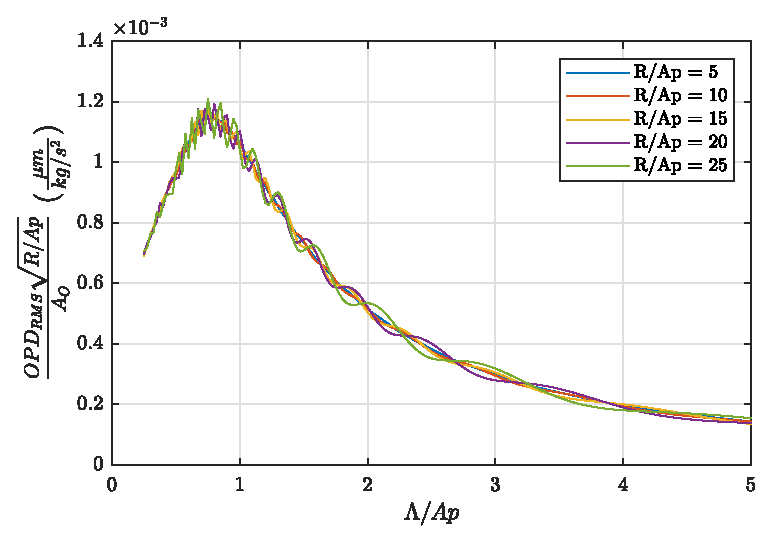
\includegraphics{../matlab/03_aero_optics_acoustics/spherical_sample.eps}
  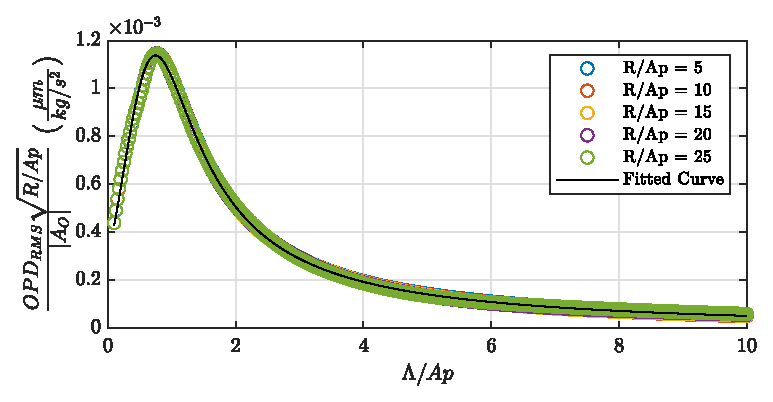
\includegraphics{../matlab/03_aero_optics_acoustics/spherical_sample_win.eps}
  \caption{Theoretical time-averaged $\opdrms$ for a spherical acoustic wave. The top plot shows a perfect spherical acoustic signal integrated over $\pm$5-m. The bottom plot shows has a Tukey window applied along the beam length to partially emulate source directivity which significantly reduces the measured oscillations.}
  \label{fig:03_spherical_sample}
\end{figure}
The top plots shows the expected optical disturbance ratio, $\opdrms/|A_0|$, for a perfectly spherical acoustic field measured over the beam length.
With the exception of some oscillations that are caused by end effects in the integration.
The oscillations can be greatly reduced by using a windowing function in the z-direction such as a Hanning or Tukey window which also can be used to roughly model directivity of the speaker's acoustic emission as shown in the bottom plot.
While this plot was calculated with a single aperture diameter, the general trend holds for all other aperture diameters that were tested, the only effect was the size and width of the oscillations.

The peak of the optical disturbance ratio, $\opdrms/|A_0|$, is located at $\Lambda/Ap\approx0.75$ for a circular aperture.
The signal is reduced above this value due to aperture filtering and below this value because the shorter wavelength have a reduced distance before alternating high and low index-of-refraction regions reduce the optical path difference.
When the acoustic source point is sufficiently far enough away from the measurement beam, $R/Ap\geq2$, the optical disturbance ratio, $\opdrms/|A_0|$ when multiplied by $\sqrt{R/Ap}$, can be collapsed onto a single curve for a range of $\Lambda/Ap$ of 0.1 to 10.
Above $\Lambda/Ap=10$ the curves start to diverge away from one another.
An approximate function fit to this data is
\begin{equation}
  \frac{\opdrms\sqrt{R/Ap}}{|A_0|} \approx \frac{p_1(\Lambda/Ap)^3+p_2(\Lambda/Ap)^2+p_3(\Lambda/Ap)+p_4}{(\Lambda/Ap)^3+q_1(\Lambda/Ap)^2+q_2(\Lambda/Ap)+q_3}
  \label{eqn:03_spherical_sample_fit}
\end{equation}
with coefficient values shown Table \ref{tab:03_speherical_sample_coeff}.
This functional fit has a $R^2$ value of 0.9991.
\begin{table}
\centering
\caption{Curve fit values for Figure \ref{fig:03_spherical_sample} and Equation \ref{eqn:03_spherical_sample_fit}}
\input{../matlab/03_aero_optics_acoustics/spherical_sample_win.txt}
\label{tab:03_speherical_sample_coeff}
\end{table}


\subsubsection{Measurement of a Spherical Acoustic Wave with an Optical Beam}
A small benchtop experiment was used to compare the simultaious optical and microphone measurements of an acoustic field from a speaker as shown in the measurement plane in Figure \ref{fig:03_speaker_test}.
\begin{figure}
  \centering
  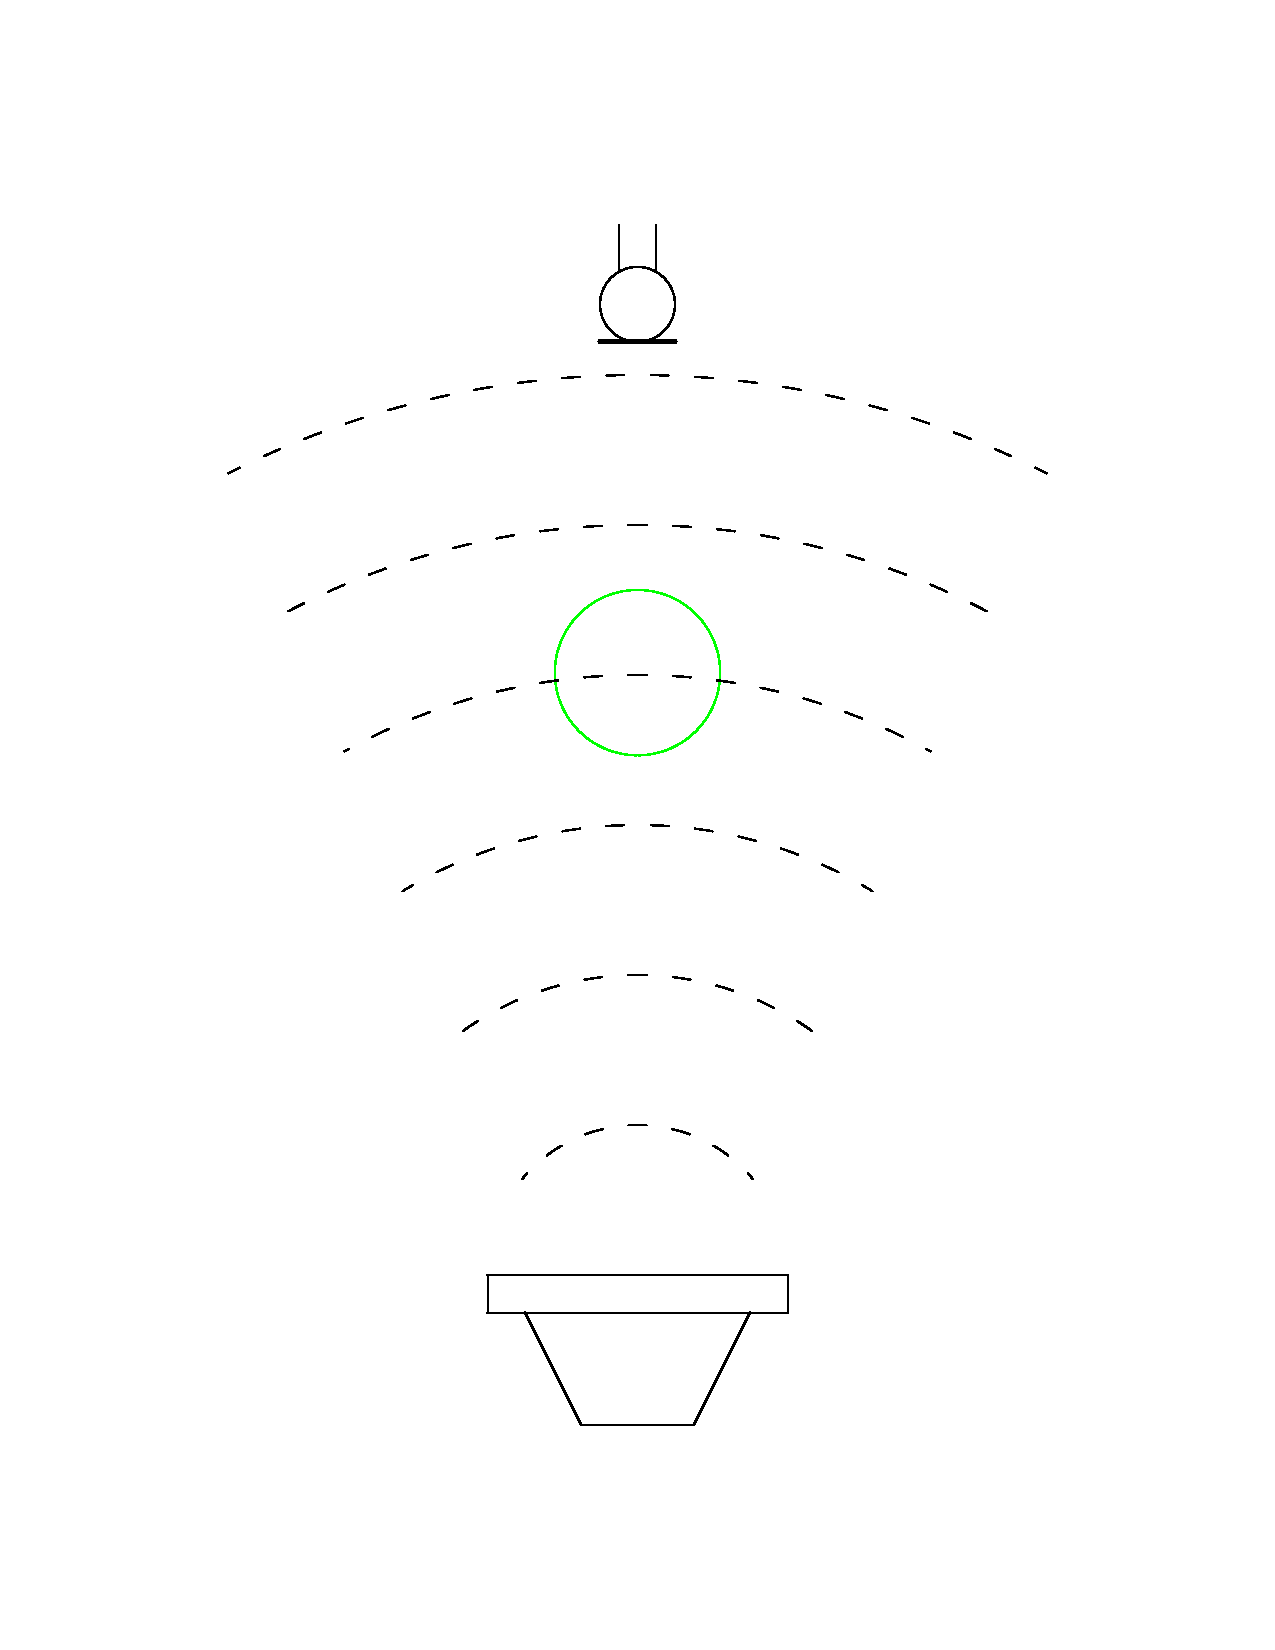
\includegraphics[width=3.5in,clip,trim=100 100 100 100]{../cad/speak_test.pdf}
  \caption{Spherical acoustic wave measurement test.}
  \label{fig:03_speaker_test}
\end{figure}
The distance from center of the beam to the speaker was 102-mm with a beam diameter of 28-mm.
A Br\"uel \& Kj\ae r model 7016B microphone was placed directly over the speaker at a distance of 158-mm.
The speaker in use was Peerless model XT25SC90-04 \cite{Peerless-XT25SC90-04-1} which has a fairly flat on-axis response from 1-kHz to 40kHz.
\cite{Bruel-Kjaer-2690}

The wavefront measurements system utilized in these measurements is similar to that shown in Figure \ref{fig:02_typical_wavefront_system} except there was no primary telescope.
The speaker was located in the center of the measurement region which was about 2-feet in length and the reimaging telescope reduced the beam diameter by a factor of two and reimaged the return mirror.
Optical wavefronts and microphone measurements were taken at 49-kHz.
The speaker was sinusoidally excited at three different frequencies (9, 14, and 18-kHz) at a variety of voltages.

The absolute value of the pulsating field strength, $|A_0|$, was calculated two different ways.
The power spectra of the microphone data was used to calculate the average $p_{rms}$ at the excitation frequency and the pulsating field strength using Equation \ref{eqn:03_spherical_pressure_rms}.
The optical wavefront was bandpass filtered at the excitation frequency using a process that will be disscussed in Chapter \ref{chap:06}.
The time averaged $\opdrms$ was used to calclate the pulsating field strength using Equation \ref{eqn:03_spherical_sample_fit}.

The results of these measurements of the pulsating field strength is shown in Table \ref{tab:03_speherical_measurement}.
The differences between the two techniques for measuring the pulsating field strength were typically with 9-11\%, with one case being at 15.5\%.
With the exception of the highest excitation case at 9-kHz, the differences between the to techniques was fairly constant for each frequency group.
For the 9-kHz cases, the wavefront estimated the pulsating field strength to be higher than the microphone estimated value.
While for the 14 and 18-kHz cases the microphone estimated the value to be higher.
Some of these differences maybe attributed to the frequency response of the microphone.
\begin{table}
  \centering
  \caption{Comparison of microphone and wavefront computation of $|A_0|$}
  \input{../matlab/03_aero_optics_acoustics/spherical_measurement.txt}
  \label{tab:03_speherical_measurement}
\end{table}

Measured and simulated wavefronts for the highest excitation cases at each frequency are shown in Figure \ref{fig:03_spherical_plot}.
\begin{figure}
  \centering
  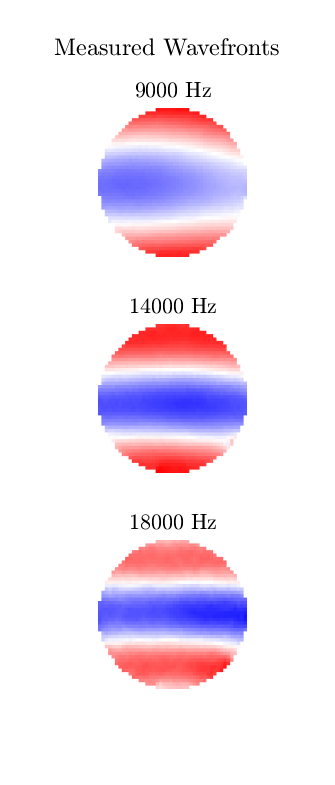
\includegraphics{../matlab/03_aero_optics_acoustics/spherical_plot_measured.eps}
  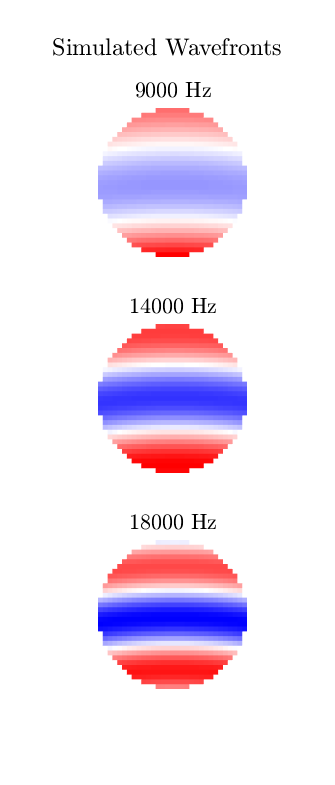
\includegraphics{../matlab/03_aero_optics_acoustics/spherical_plot_simulated.eps}
  \caption{Comparison of some of the measured wavefronts and simulated ones.}
  \label{fig:03_spherical_plot}
\end{figure}
The 9-kHz case shows some anomalies on the measured wavefront on the right side, diviating from spherical wave significantly likely contributing the significantly higher estimated pulsating field strength value when compared to the microphone estimate.
The 14 and 18-kHz cases show some remarkable agreement between the measured and simulated images.
Optical wavefront measurements can be utilized for making non-intrusive acoustic field measurements espically when the acoustic field is simple.



\section{Estimating the Acoustic Field Inside the Test-Section}



\subsection{Mode Marching Process}
\begin{enumerate}
  \item Start with a known or assumed source acoustic field, $p^n(x,y)$

  \item Calculate the transmitted pressure ratio
  \begin{itemize}
    \item Traveling with subsonic flow
      \begin{equation}
        \frac{p^t}{p^i} = \left(\frac{1+M_n}{1+M_{n+1}}\right)\left(\frac{2M_{n+1}}{M_n+M_{n+1}}\right)\left(\frac{X_{n,n}}{X_{n,n+1}}\right)\left(\frac{X_{n,n}}{X_{n+1,n+1}}\right)^{1/(\gamma-1)}
      \end{equation}
    \item Traveling against subsonic flow
      \begin{equation}
        \frac{p^t}{p^i} = \left(\frac{1-M_n}{1-M_{n+1}}\right)\left(\frac{2M_{n+1}}{M_n+M_{n+1}}\right)\left(\frac{X_{n,n}}{X_{n,n+1}}\right)\left(\frac{X_{n,n}}{X_{n+1,n+1}}\right)^{1/(\gamma-1)}
      \end{equation}
    \item Where
      \begin{equation}
        X_{a,b} = 1+\frac{\gamma-1}{2}M_aM_b
      \end{equation}
  \end{itemize}

  \item March acoustic field to next axial step,
    \begin{equation}
      p^{n+1}(x,y) = p^{n}(x,y)\frac{p^t}{p^i}\exp\{j(\omega t\mp k_{zm}^\pm z)\}
    \end{equation}

  \item Best-fit set of local duct modes coefficients, $C_m$, to acoustic field $p^{n+1}(x,y)$

  \item Calculate new acoustic field from duct mode and repeat from step 2
    \begin{equation}
      p^n(x,y) = \sum_{m=0}^{M} C_m\cdot p_m(x,y)
    \end{equation}

  \item When the end point is reached, step inlet acoustic field (rotate fan) and repeat
\end{enumerate}

% !TEX root = catron-dissertation.tex
\epstopdfsetup{outdir=./images/04_basic_filtering/}

\chapter{Basic Wavefront Filtering Techniques}
\label{chap:wavefront_filtering}
This chapter will examine some basic wavefront filtering techniques for removal of undesired content from an optical wavefront measurement using a synthetically generated wavefront.
These basic filtering techniques are based on performing a dispersion analysis in order to compute the optical wavefronts spectral content in both time and space.
These techniques are primarily designed for preforming a quick analysis of measured data with some knowledge of the corruption that is present or some user intervention.
It is also likely to remove some desired wavefront components and/or retain some of the measurement corruption.

\section{Dispersion Analysis}
The dispersion analysis as used in this paper is a method for calculating the power spectral density of an optical wavefront in both time and space.
The result for a 2-D optical wavefront that varies over time is 3-D scalar array that lays in temporal (Hz) and spacial ($m^{-1}$) frequency space.
Structures in the dispersion plot lay along a plane that represents its velocity in both $x$ and $y$ directions.
A simple visualization of this is shown in Figure \ref{fig:04_simple_dispersion}.
\begin{figure}
  \centering
  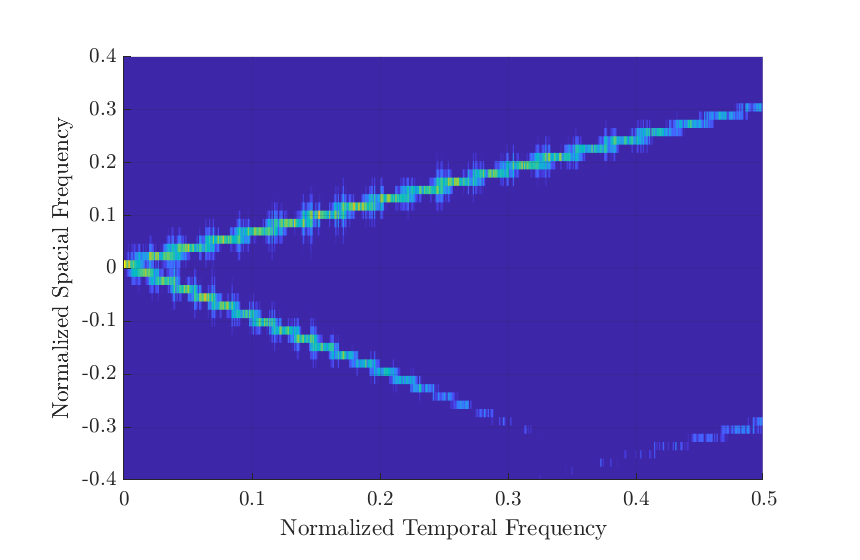
\includegraphics{../matlab/04_basic_filtering/simple_dispersion.eps}
  \caption{A simplified dispersion plot.  Simulation of two broadband plane waves traveling in opposite directions through a 1-D wavefront.}
  \label{fig:04_simple_dispersion}
\end{figure}
This simple representation is a simulated 1-D wavefront (containing spatial data in only one dimension) that consists of two broadband planar wave structures, one that travels in the negative x-direction while the other in the positive x-direction at 5/3 the speed.
The slope of the structures are inversely related to their velocities when represented with the temporal frequency along the x-axis.
The wave structure traveling in the positive x-direction has much higher frequency content, higher so than the temporal Nyquist frequency and gets aliased into the negative x-direction.
Depending on the filtering methods used, this aliased information can be added no to both ends of the dispersion array in the temporal direction to artificially increase the temporal sample rate of the system.
In this simplified version with the exception of the aliased data and overlap region, these two flow structures can easily be separated into two distinct wavefront components when analyzing the wavefront in frequency space.

This dispersion plot can be displayed in a different way, see Figure \ref{fig:04_simple_dispersion_vel}, such that the y-axis represents the velocity of structure if a linear trend between the spatial and temporal frequencies and velocity is assumed.
\begin{figure}
  \centering
  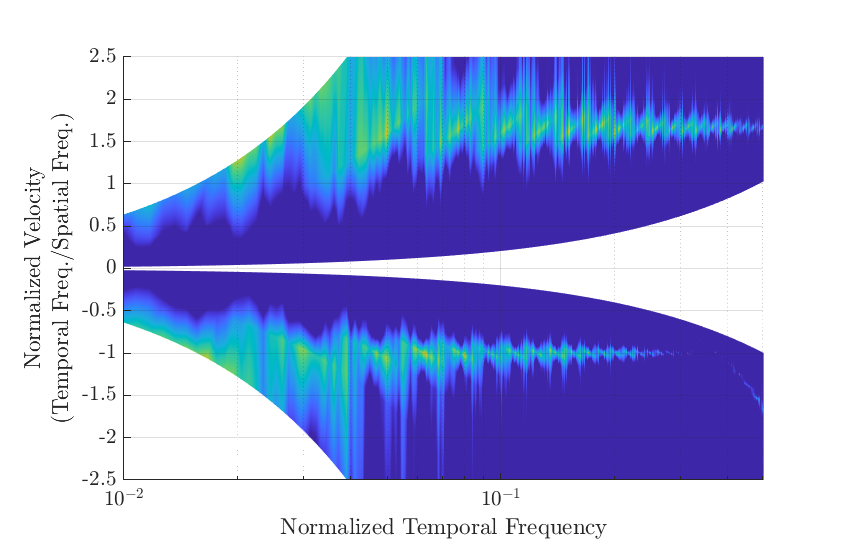
\includegraphics{../matlab/04_basic_filtering/simple_dispersion_vel.eps}
  \caption{Alternative representation of the simplified dispersion plot.  Simulation of two broadband plane waves traveling in opposite directions through a 1-D wavefront.}
  \label{fig:04_simple_dispersion_vel}
\end{figure}
Here both waves that are traveling in either direction are clearly discernible, even to low frequencies and allows for the direct reading of the velocity of the group of waves.
One big issue with this representation is the aliased data, which does not show up as a constant velocity as could interpret the standard dispersion plot seeing that both lines have the same slope although different y-intercept.

While these plots only show information in the x-spatial/temporal plane, the analysis can be performed in the y-spatial/temporal plane or even 3-D representations as shown in Figure \ref{fig:04_dispersion_real}.
\begin{figure}
  \centering
  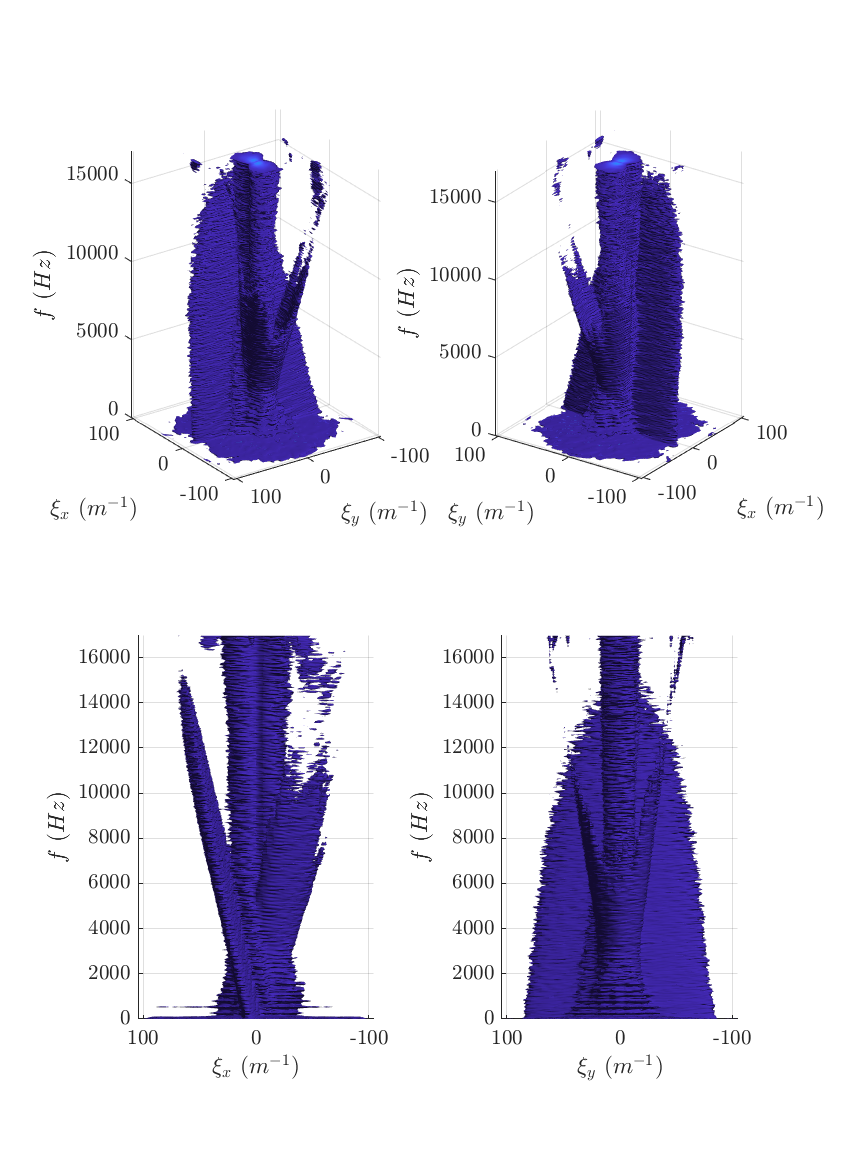
\includegraphics{../matlab/04_basic_filtering/dispersion_real.eps}
  \caption{Dispersion analysis isosurface at a value of $10^{-13}$ $\mu m^2/Hz/m^{-2}$ from two different views.  The isosurface encompasses 99.5\% of the energy of the optical disturbances.}
  \label{fig:04_dispersion_real}
\end{figure}
This figure shows an isosurface, which encompasses about 99.5\% of the energy, of some measured data where several different prominent structures.
The wing shaped structure contains the aero-optical signal of the boundary layer and free-stream turbulence.
The figure-eight shaped structure is measurement noise, while the partial cone is the acoustic duct modes inside the test section.
The large structure near zero-temporal frequency is a combination of vibrations and acoustic contamination, especially around the blade-pass frequency and associated harmonics.

\section{Dispersion Calculation}
As the dispersion analysis is just an extension of the typical power spectra calculation,
\begin{equation}
  S_{xx} = \frac{|\fft(x(t))|^2}{N\cdot f_{samp}} \textrm{,}
  \label{eqn:04_basic_sxx}
\end{equation}
to multiple dimensions, where $\fft$ is the Fast Fourier Transform function, $N$ is the number of points in the transform, $f_{samp}$ is the sample rate, and $S_{xx}$ is the double sided power spectra.
Note, that this form of the equation is for use with MATLAB's way of computing the FFT.
The frequency range goes from $0$ to $f_{samp}\cdot(1-1/N)$ in steps of $f_{samp}/N$ and if the function \lstinline{fftshift} is used on the \lstinline{fft} output the range is augmented to go from $-f_{samp}/2$ to $f_{samp}\cdot(1/2-1/N)$ with the same frequency step size.

Because the FFT calculation assumes the signal is periodic, spectral leakage can occur when the signal is not an integer number of periods long.
If minimize this spectral leakage windows are employed which typically force the end points of the signal to zero so the spectral leakage is greatly reduced.
The Hann window,
\begin{equation}
  w(t) = 1/2\left[1-\cos\left(\frac{2\pi t}{T}\right)\right] \textrm{,}
  \label{eqn:04_hann_window}
\end{equation}
is one of the more commonly used windowing functions where $w(t)$ is the window function, $t$ is the time at a given sample, and $T$ is the total sample time.
Since the windowing of a data set changes the signal energy some correction is needed to be applied.
For an arbitrary windowing function this correction factor, $c_w$, is
\begin{equation}
  c_w = \frac{1}{\sqrt{\sum w^2(t)/N}} \textrm{.}
  \label{eqn:04_window_correction}
\end{equation}
For a Hann window this correction factor approaches $\sqrt{8/3}$ as $N$ goes to infinity.
When the equaiton \ref{eqn:04_basic_sxx} is combined with a windowing function and associated correction the double sided power spectra equation in one dimension becomes
\begin{equation}
  S_{xx} = c_w\cdot\frac{|\fft\{x(t)\cdot w(t)\}|^2}{N\cdot f_{samp}} \textrm{.}
  \label{eqn:04_windowed_sxx}
\end{equation}
A simple MATLAB function for computing the power spectra of an one-dimension signal with an arbitrary windowing function is shown in Listing \ref{code:sc_simpleSXX}.

For measurements with multiple spatial and temporal dimensions, such as typical optical wavefronts with two spatial dimensions at a discrete time interval, the Fast Fourier Transform is just applied $n$-times where $n$ is the total number of dimensions, with each application in a different dimension,
\begin{equation}
  \fftn(x) = \fft(\fft(\cdots\fft(\fft(x,1),2)\cdots,n-1),n) \textrm{,}
  \label{eqn:04_fftn}
\end{equation}
where $\fft(x,n)$ is the Fast Fourier Transform of $x$ in the $n^{th}$ dimension.
For a $n$-dimensional array the power spectra the function becomes,
\begin{equation}
  \mathbf{S_{xx}} = c_w\cdot\frac{|\fftn\{f(\mathbf{x})\cdot w(\mathbf{x})\}|^2}{\prod{\overrightarrow{N}\cdot \overrightarrow{f}_{samp}}} \textrm{,}
  \label{eqn:04_sxxn}
\end{equation}
where $\mathbf{S_{xx}}$ is the $n$-dimensional power spectra array or dispersion array, $f(\mathbf{x})$ is a $n$-dimensional set of data, $w(\mathbf{x})$ is a $n$-dimensional windowing function, $\overrightarrow{N}$ is a vector denoting the number of elements in each dimension, $\overrightarrow{f}_{samp}$ is a vector denoting the sample rate in each dimension, and
\begin{equation}
  c_w = \frac{1}{\sqrt{\sum w^2(\mathbf{x})/\prod{\overrightarrow{N}}}} \textrm{.}
  \label{eqn:04_windown}
\end{equation}
A simple MATLAB code for calculating the dispersion of $x$ with an arbitrary windowing function is shown in Listing \ref{code:sc_simpleSXXn}.

The optical wavefronts used throughout this paper are round apertures with no additional obscurations and is constant throughout the sample period.
This allows the windowing function to be split into two separate components,
\begin{equation}
  w(\mathbf{x}) = w_t(t)\cdot w_s(x,y) \textrm{,}
  \label{eqn:04_window_sep}
\end{equation}
the temporal windowing function, $w_t(t)$, and the spatial windowing function, $w_s(x,y)$.
Both the temporal and spatial windowing functions used in this paper are Hann windows.
The temporal window used the function shown in Equation \ref{eqn:04_hann_window}, while the spatial windows used a modified version based on the normalized radius, $\rho_N$, of the aperture such that at the center of the aperture the weighting was one and the edge the weighting was zero and remained zero outside to the aperture,
\begin{equation}
  w_s(\rho_N) =
  \begin{cases}
    \frac{1+\cos(\pi\cdot\rho_N)}{2} & \textrm{if } \rho_N < 1 \\
    0 & \textrm{otherwise.}
  \end{cases}
  \label{eqn:04_window_space}
\end{equation}

For an arbitrary shaped aperture a windowing function can be computed by finding the minimum distance from any point within the aperture to a point outside of the aperture,
\begin{equation}
  d_{min}(x,y) = \min\left\{\sqrt{(x-x_{O})^2+(y-y_{O})^2}\right\} \textrm{,}
\end{equation}
where $O$ denotes the set of points outside of the aperture.
This distance is then normalized by the maximum value.
The windowing function is just a slight modification of the Hann window function again,
\begin{equation}
  w_s(x,y) = \frac{1+\cos\left\{\pi\cdot\left(1-d_{min}^{norm}(x,y)\right)\right\}}{2} \textrm{.}
\end{equation}

% \begin{equation}
%   \pi\cdot\left(1-\frac{d(x,y)}{\max\{d(x,y)\}}\right)
% \end{equation}

\section{Synthetic Wavefront Generation}
In order to best understand how some basic filters preform on a set of data, a fully known synthetic wavefront was generated such that all the various components could be generated separately with the combined product filtered and compared to the synthetic wavefront containing only relevant aero-optical data.
This is done by creating an input dispersion plot where each source component is separately generated with parameters that can be modified to alter the output signal as necessary.
Signals that are assumed to be statistically independent are converted into dimensional space separately and then summed together, while signals that are assumed to be related to one another (sound and vibration components) are summed together in frequency space.
Figure \ref{fig:04_synthetic_dispersion_input} shows the input dispersion plot with each signal component separately colored.
\begin{figure}
  \centering
  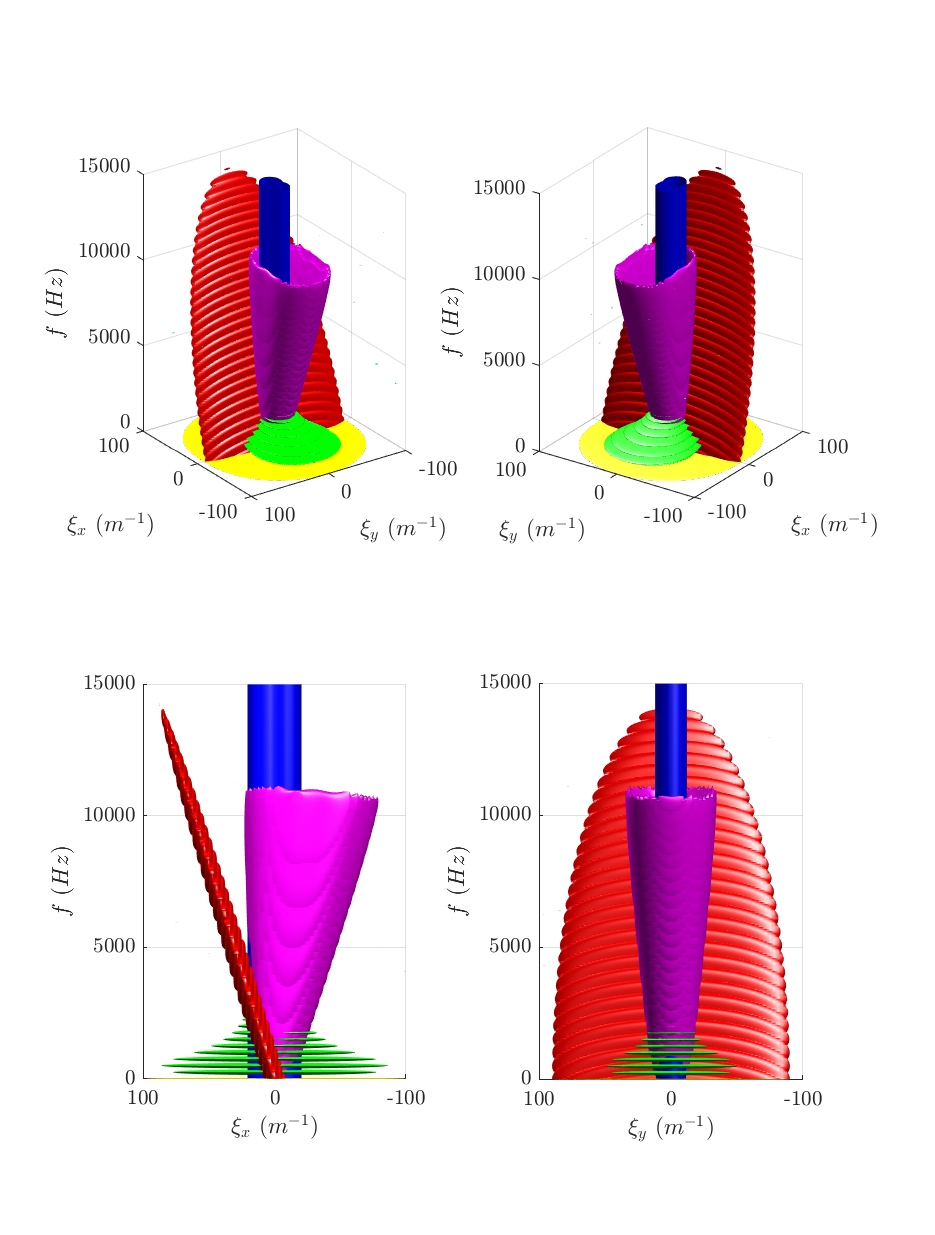
\includegraphics{../matlab/04_basic_filtering/synthetic_wavefront.eps}
  \caption{Synthetic wavefront input dispersion plot of an aero-optical signal and various signal corruption components.  The aero-optical signal is shown in red, the stationary modes in blue, duct acoustics in magenta, blade-passing frequency related corruption in green, slowly varying mean-lensing in yellow, and background in cyan.}
  \label{fig:04_synthetic_dispersion_input}
\end{figure}
The aero-optical signal is shown in red, the stationary modes in blue, duct acoustics in magenta, blade-passing frequency related corruption in green, slowly varying mean-lensing in yellow, and background in cyan.

Wavefronts were generated approximate the sample conditions in that the data presented in Figure \ref{fig:04_dispersion_real} were measured with.
The sample rate was 200 m$^{-1}$ with 64 ($2^6$) samples in the spatial dimensions and 30,000 Hz with 8192 ($2^{13}$) samples in the temporal dimension.
The speed of sound was chosen to be 340 m/s, with a Mach number of 0.6, and a boundary layer velocity of 163.2 m/s ($0.8U_\infty$).

The general process of developing most of the component signals was to determine an approximate shape, normalize it in the appropriate dimensions, and scale the result by using a function derived from a hyperbola,
\begin{equation}
  \frac{\log_{10}(WF)-b}{b^2}-\frac{\xi_{\rho_N}^2}{a^2} = 1 \textrm{,}
  \label{eqn:04_scaling_hyperbola}
\end{equation}
such that the signal strength at unity of the normalized radial frequency, $\log_{10}(WF(\xi_{\rho_N}=1))$, and the limiting slope, $a/b$, are inputs.
This results in the signal strength of the wavefront being
\begin{equation}
  \log_{10}(WF) = b-\sqrt{\frac{\xi_{\rho_N}^2}{m^2}+b^2} \textrm{,}
  \label{eqn:04_wavefront_strength}
\end{equation}
where
\begin{equation}
  b = \frac{1}{2\log_{10}(WF(\xi_{\rho_N}=1))}\cdot\left(\log_{10}(WF(\xi_{\rho_N}=1))^2-\frac{1}{m^2}\right) \textrm{.}
  \label{eqn:04_wavefront_strength_b}
\end{equation}
The code used to generate the synthetic wavefront used in this section as well as it inputs are shown in Listing \ref{code:sc_synthetic_wavefront}.

\subsection{Aero-Optical Signal}
The aero-optical signal which is approximating an optical beam passing through two boundary layers normal to the wall.
This signal was approximated by creating an ellipsoid in the plane of the feature's velocity and normalizing the radius by some arbitrary factors to roughly match the shape of the measured dispersion plot shown in Figure \ref{fig:04_dispersion_real}.
The dispersion magnitude was then calculated by applying Equation \ref{eqn:04_wavefront_strength}, with relevant code shown on Lines 19-30 of Listing \ref{code:sc_synthetic_wavefront}.
In Figure \ref{fig:04_synthetic_dispersion_input} the aero-optical signal is shown in red.
% \lstinputlisting[label=code:04_synthetic_ao, linerange={19-30}, numbers={left}, caption={Code for generating a synthetic dispersion plot of an aero-optical source.}, language=Matlab]{../matlab/04_basic_filtering/synthetic_wavefront.m}

\subsection{Stationary Mode Signals}
The stationary modes in Figure \ref{fig:04_dispersion_real} appear to be temporally white-noise with the spatial frequencies forming an epicycloid of $k=2$.
This shape was further simplified using a single trigonometric function to represent the normalization function of the radial spatial frequency,
\begin{equation}
  \xi_{\rho_N} = \frac{\xi_\rho}{\xi_{\rho_0}\sqrt{10-6\cos{(2\xi_\theta)}}} \textrm{,}
\end{equation}
this makes an epicycloidal like shape which has a smooth derivative.
This dispersion component is shown in blue in Figure \ref{fig:04_synthetic_dispersion_input} and the relevant code shown in Lines 61-66 of Listing \ref{code:sc_synthetic_wavefront}.
% \lstinputlisting[label=code:04_synthetic_sn, linerange={61-66}, numbers={left}, caption={Code for generating a synthetic dispersion plot of the stationary mode disturbances.}, language=Matlab]{../matlab/04_basic_filtering/synthetic_wavefront.m}

\subsection{Sound \& Vibration Signals}
The sound \& vibrating component signals are comprised of two parts.
The first of these if the blade-passing frequency and harmonic disturbances (shown in green in Figure \ref{fig:04_synthetic_dispersion_input}) and the second in the acoustic duct modes (shown in magenta).
Like the stationary modes, the blade-passing frequency disturbances were modeled with the simplified epicycloid narrow-band disc and each harmonic was modulated by using a low-pass filter offset to the blade-passing frequency.
The code for the blade-passing frequency disturbances is shown in Lines 97-113 of Listing \ref{code:sc_synthetic_wavefront}.
% \lstinputlisting[label=code:04_synthetic_bpf, linerange={97-113}, numbers={left}, caption={Code for generating a synthetic dispersion plot of the blade-passing frequency disturbances.}, language=Matlab]{../matlab/04_basic_filtering/synthetic_wavefront.m}

The acoustic duct mode disturbances form a cone which in the $f-\xi_x$ plane is defined by the lines $u\pm c$, while in the $f-\xi_y$ plane is defined by the speed of sound.
At each temporal frequency step an ellipse was defined based on the the constraining lines and the distance to that ellipse used to calculate a normalized radial frequency.
The strength of the disturbance was decreased logarithmically in temporal frequency as shown in the code in Lines 183-200 of Listing \ref{code:sc_synthetic_wavefront}.
% \lstinputlisting[label=code:04_synthetic_cone, linerange={183-200}, numbers={left}, caption={Code for generating a synthetic dispersion plot of the acoustic duct mode disturbances.}, language=Matlab]{../matlab/04_basic_filtering/synthetic_wavefront.m}

\subsection{Mean Lensing Signal}
The mean-lensing signal (shown in yellow in Figure \ref{fig:04_synthetic_dispersion_input}) uses a stretched version of the simplified epicycloid and represents the slowly varying spatial disturbance.
The relevant code is shown on Lines 144-152 of Listing \ref{code:sc_synthetic_wavefront}.
% \lstinputlisting[label=code:04_synthetic_zero, linerange={144-152}, numbers={left}, caption={Code for generating a synthetic dispersion plot of the mean lensing disturbance.}, language=Matlab]{../matlab/04_basic_filtering/synthetic_wavefront.m}

\subsection{Background Noise Signal}
The background noise disturbance (with a few small spots shown in cyan in Figure \ref{fig:04_synthetic_dispersion_input}) was the only component that did not use the hyperbola to scale the signal but instead was just normally distributed random noise with a mean noise level and deviation as inputs.
The relevant code is shown in Lines 230-234 of Listing \ref{code:sc_synthetic_wavefront}.
% \lstinputlisting[label=code:04_synthetic_back, linerange={230-234}, numbers={left}, caption={Code for generating a synthetic dispersion plot of the mean lensing disturbance.}, language=Matlab]{../matlab/04_basic_filtering/synthetic_wavefront.m}

\subsection{Synthetic Wavefront Creation}
A synthetic signal can be created from a power spectra by solving for $x$ in Equation \ref{eqn:04_basic_sxx} and using the Inverse Fast Fourier Transform,
\begin{equation}
  x(t) = \real\left[\ifft\left\{\sqrt{S_{xx}\cdot N\cdot f_{samp}}\cdot\exp{i\phi}\right\}\right] \textrm{,}
  \label{eqn:04_ifft}
\end{equation}
where $\real$ is the real component and $\phi$ is a random set of phases for each point in the measurement space.
As shown previously this relation can be extended into $n$-dimensions,
\begin{equation}
  f(\mathbf{x}) = \real\left[\ifftn\left\{\sqrt{\mathbf{S_{xx}}\cdot\prod{\overrightarrow{N}\cdot \overrightarrow{f}_{samp}}}\cdot\exp{i\mathbf{\phi}}\right\}\right] \textrm{.}
  \label{eqn:04_ifftn}
\end{equation}
Care should be taken when constructing the random set of phases, as the zero-frequency component has zero phase and the phases on either side of it are conjugates of one another.
The code for creating a wavefront from a dispersion plot is shown in Lines 336-340 of Listing \ref{code:sc_synthetic_wavefront} and is specifically creating the wavefront for the aero-optical signal but other signals are generated using the same basic code.
Note that the first three lines are to get the set of phases properly configured that creates conjugate phases rotated about the origin.
% \lstinputlisting[label=code:04_synthetic_wf, linerange={336-340}, numbers={left}, caption={Code for generating a synthetic wavefront from a dispersion plot.}, language=Matlab]{../matlab/04_basic_filtering/synthetic_wavefront.m}

It was assumed that the aero-optical signal, the stationary modes, and the background noise were statistically independent of one another and the sound \& vibration combination of modes and as such could be separately transformed into physical space.
While the components of the sound \& vibration sources, the blade-passing frequency, the acoustic cone, and the mean-lensing, were assumed to be replated to one another and thus were summed together in frequency space prior to being transformed into physical space.
Once the separate components were in physical space the total wavefront was obtained by summing up the separate components with the aero-optical signal being a separately saved along side the total wavefront.
Some frames from the synthetic wavefront are shown in Figure \ref{fig:04_synthetic_frames} with the total wavefront shown on top and the aero-optical only signal shown of the bottom.
\begin{figure}
  \centering
  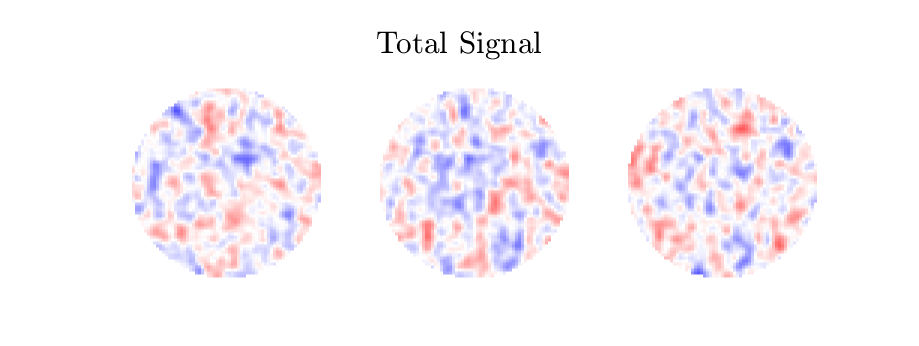
\includegraphics{../matlab/04_basic_filtering/synthetic_frames_total.eps}
  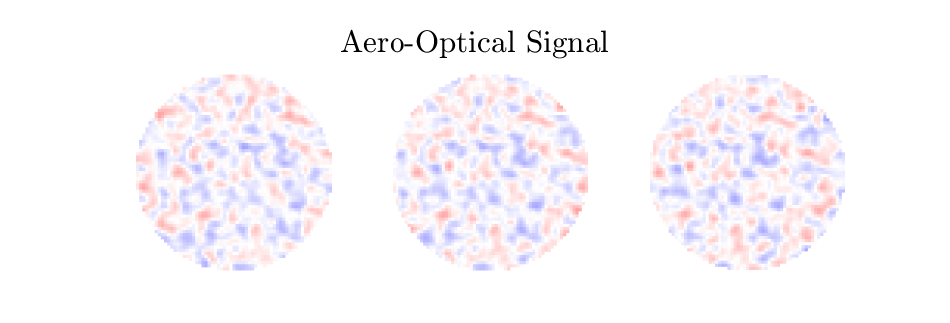
\includegraphics{../matlab/04_basic_filtering/synthetic_frames_ao.eps}
  \caption{Sample frames from the synthetic wavefront with the total wavefront signal on top and the aero-optical only signal bottom.  Flow is from right to left.}
  \label{fig:04_synthetic_frames}
\end{figure}
Flow if from right to left.
The aero-optical signal is often times noticeable in the total wavefront signal but can be easily overpowered by the various contamination sources.

A dispersion plot of the total synthetic wavefront is shown in Figure \ref{fig:04_dispersion_synthetic}.
\begin{figure}
  \centering
  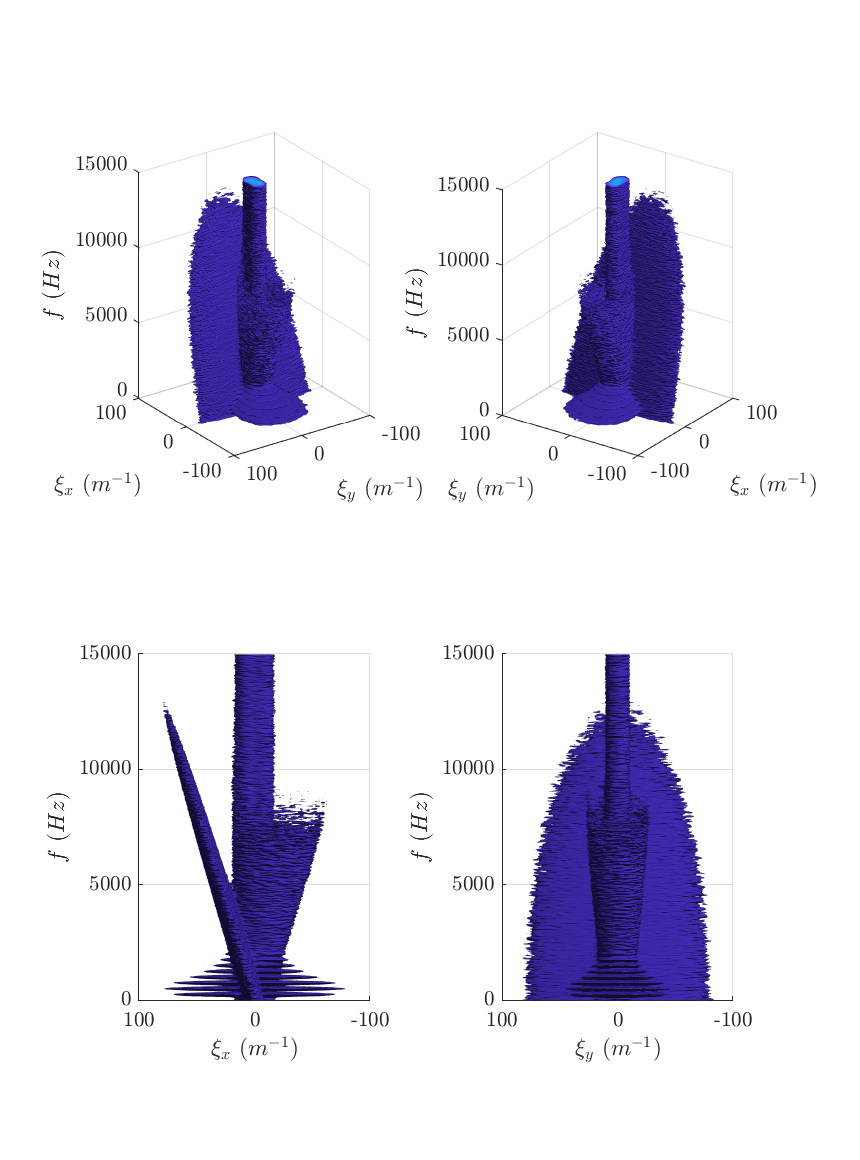
\includegraphics{../matlab/04_basic_filtering/dispersion_synthetic.eps}
  \caption{Synthetic wavefront output dispersion plot of an aero-optical signal and various signal corruption components.}
  \label{fig:04_dispersion_synthetic}
\end{figure}
In this view the aero-optical signal is more noticeable but there still remains some significant overlap with the various contamination sources.
While the mean-lensing component is not as visable in this isosurface, the rest of the dispersion plot in a good representation of the input dispersion plot shown in Figure \ref{fig:04_synthetic_dispersion_input}.
The total synthetic wavefront has a spatial time-averaged rms of $0.0112\pm0.0006\mu m$ with the aero-optical only signal having a spatial time-averaged rms of $0.0073\pm0.0003\mu m$.
The measured wavefront presented in Figure \ref{fig:04_dispersion_real} had a spatial time-averaged rms of $0.0874\pm0.0263\mu m$.
The overall spatial rms of the synthetic wavefront is $12.8\%$ when compared to the measured wavefront indicating that the algorithms used to generate the wavefront are not representative of reality and can provide a future path of research in order to produce more realistic synthetic wavefronts.

\subsection{Comparison to Measured Data}

\section{Filtering Basics}
A filter is a function, $G(\mathbf{\omega})$, that describes the gain a signal will experience in frequency space.
In the simplest case, the filtered signal is the inverse Fourier transform of the gain multiplied by the Fourier transform of the signal.
Additionally, a windowing function, $W(\mathbf{x})$, can be used to help suppress finite sampling effects,
\begin{equation}
  f_F(\mathbf{x}) = \real\left(\frac{\ifftn[G(\mathbf{\omega})\cdot\fftn\{f(\mathbf{x})\cdot W(\mathbf{x})\}]}{W(\mathbf{x})}\right) \textrm{,}
  \label{eqn:04_filter_function}
\end{equation}
where $f$ is the signal function and $f_F$ is the filtered signal.
Depending on the windowing function some data could be destroyed during this process if there is a zero present due to a divide by zero.

A basic MATLAB code for applying a filter to a wavefront using a separate function for both generating and applying the gain function which is presented in Listing \ref{code:sc_basic_wavefront_filters}.
% \lstinputlisting[label=code:04_basic_filter_process, linerange={5-13}, numbers={left}, caption={Code for applying a filter to a wavefront with a windowing function.}, language=Matlab]{../matlab/04_basic_filtering/basic_filter_process.m}
This code generates a windowing function as described by Equations \ref{eqn:04_hann_window}, \ref{eqn:04_window_sep}, and \ref{eqn:04_window_space}.
The temporal windowing function was generated with an additional two term such that the end point which are equal to zero could be removed to prevent the first and last frames from being destroyed due to zero being divided by zero.
Likewise the normalized radius was only allow to approach one in order to prevent the lose of any sub-apertures.
The filter presented in this code sample is a second order temporal high-pass filter with a cut-off frequency of 2000 Hz.
The function \lstinline{WFfilter} takes input based on a normalized cut-point in reference to the sample rate.

\section{Temporal Filter Methods}
The methods presented in this section are based on Butterworth filters \cite{Butterworth-1930-DvDrjKha} but could easily be extended to other types of types of filters.
The basic gain function,
\begin{equation}
  G(f) = \frac{1}{\sqrt{1+\left(\frac{f}{f_c}\right)^{\pm2n}}} \textrm{,}
  \label{eqn:04_butterworth}
\end{equation}
where $f_c$ is the cut-off frequency, $n$ is the filter order (number of filters in a series), and $\pm$ represents either a low-pass ($+$) or high-pass ($-$) filter.
In this particular formulation, only the magnitude is attenuated, circuit based Butterworth filters or their digital copies will have some variable phase attenuation as well.
Additionally, a band-pass filter can be constructed by placing a low-pass in series with a high-pass filter and a band-stop by placing the two types in parallel.

As a large portion of the wavefront contamination is at low frequencies, a high-pass filter is the most useful in temporal space for removing unwanted contamination, as shown in Figure \ref{fig:04_filter_temporal}.
\begin{figure}
  \centering
  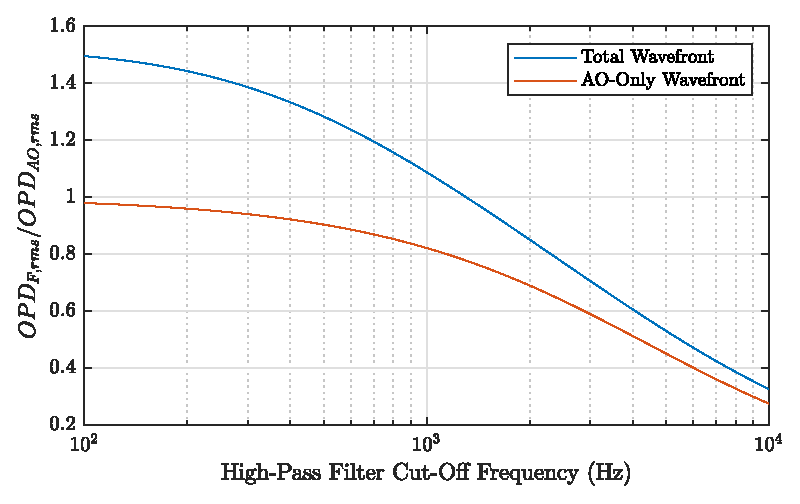
\includegraphics{../matlab/04_basic_filtering/filter_temporal.eps}
  \caption{OPD time-averaged spatial-RMS of high-pass temporal filters relative to the aero-optical only unfiltered wavefront.}
  \label{fig:04_filter_temporal}
\end{figure}
This figure shows the time-averaged spatial-RMS of both the total and aero-optical only wavefronts with various cut-off high-pass filters relative to that of the aero-optical only wavefront unfiltered.
The main thing to note is that the total wavefront ratio crosses unity between around 1200 Hz, which is about halfway between the second and third harmonic of the blade-passing frequency in this simulated wavefront.
While only ~75\% of the aero-optical signal remains, that difference is made up by the remaining contamination signal.
This can provide a very computationally cheap way estimating the aero-optical portion of the wavefront for calculations that rely on the spatial-RMS of a wavefront.
While it is easy to determine a cut-off frequency for this synthetic wavefront, a measured wavefront will likely take some knowledge or expectation of the contamination that is present in the measurement.

An example of band-pass and band-stop filtering is shown if Figure \ref{fig:04_filter_temporal_bandpass}.
\begin{figure}
  \centering
  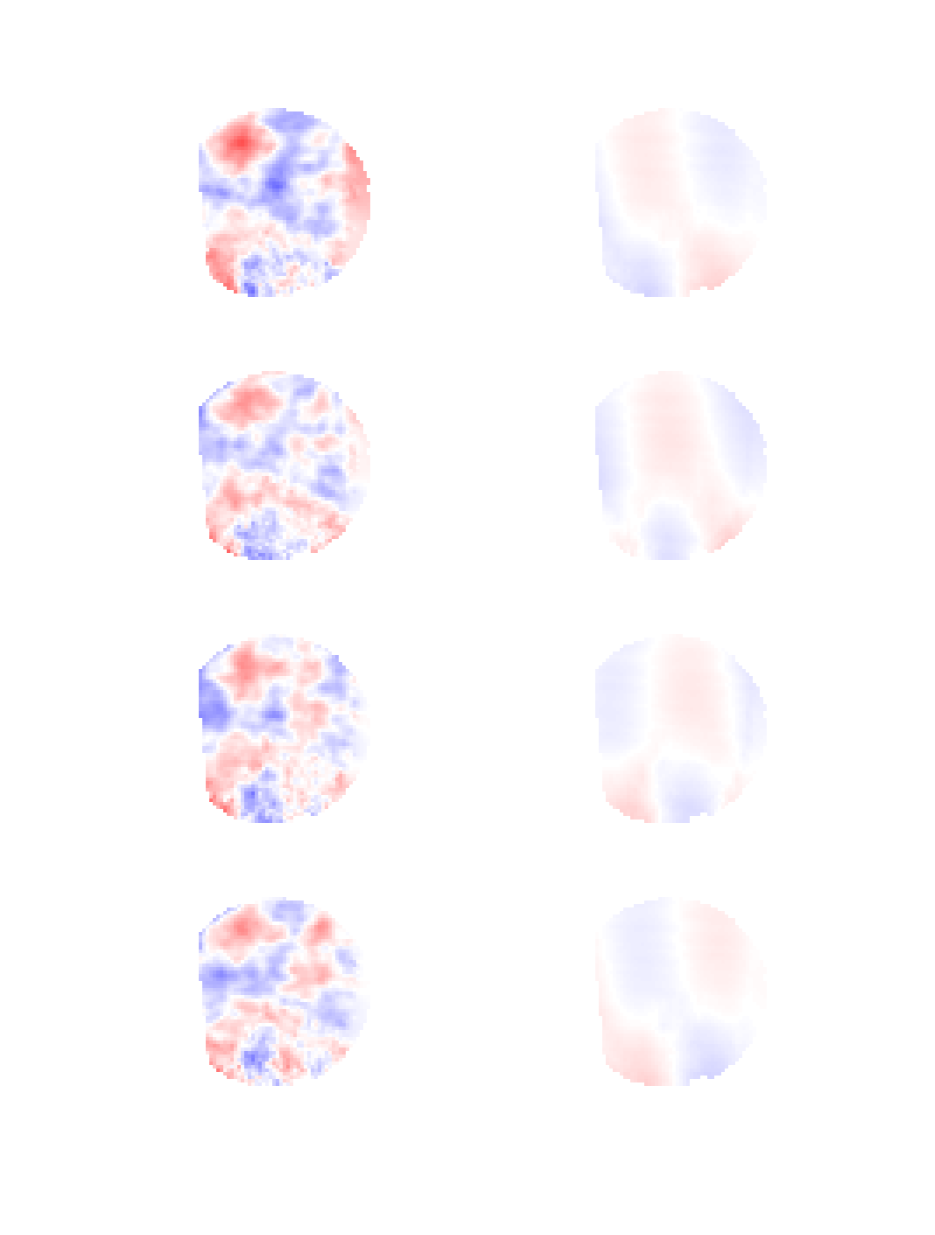
\includegraphics{../matlab/04_basic_filtering/filter_temporal_bandpass.eps}
  \caption{Measured wavefronts filtered at the blade-passing frequency (532$\pm$10 Hz).  The left column is band-stop filtered while the right is band-pass filtered.}
  \label{fig:04_filter_temporal_bandpass}
\end{figure}
The figure shows measured data that is band-stop filtered in the left column and band-pass filtered in the right column in several different frames.
The flow is from right-to-left and the band-pass filtered wavefront clearly shows upstream-moving optical disturbances associated with acoustic duct modes traveling upstream from the fan.
The band-stop shows a much slower moving optical disturbance at is in general moving in the direction of the flow but it still possess the blade-pass frequency harmonics caused optical disturbances.

One thing of note, MATLAB's builtin filter functions only work in one-dimension of frequency space so are unable to determine the direction that a signal is traveling.
They also only apply the filter to the positive frequencies and zero-out the negative ones which both halves the signal passing through the filter it also switches all disturbances to moving in the same direction.
So even for a filter that operates in one-dimension, it is best to apply the filter over both positive and negative frequencies to the n-dimensional Fourier transform in order to preserve the direction of travel of a signal.
This Additionally allows several filters to be applied in series with one another without having to perform a Fourier and inverse Fourier transform for each successive filter.
% Maybe show this in an appendix.

Some additional uses of temporal filters would be in sizing and/or designing an adaptive optics system.
A low-pass filter with a cut-off at the bandwidth of a either a fast-steering or deformable mirror would help determine the signal that a system would need to reject.
A control system may need to have the bandwidth reduced in order to keep a mirrors travel within limits.
While a high-pass filter would inform designers the remaining optical aberrations that cannot be corrected and have to be lived with.




\section{Upstream/Downstream Moving}
For the filtering of upstream and downstream moving optical disturbances a logistic function was chosen,
\begin{equation}
  f(x) = \frac{1}{1+\exp\{-kx\}} \textrm{.}
  \label{eqn:04_logistic}
\end{equation}
This function needs to be expanded into two-dimensions ($x$ and $t$) with the filter ideally returning a value of one in both the first and third quadrants and zero otherwise when wanting to obtain the disturbances moving in the direction of flow.
To accomplish this the logistic curve in each dimension is scaled and offset to output values between negative one and positive one,
\begin{equation}
  G_t(f) = \frac{2}{1+\exp\{-k_tf\}}-1
  \label{eqn:04_logistic_time}
\end{equation}
and
\begin{equation}
  G_x(\xi_x) = \frac{2}{1+\exp\{\pm k_x\xi_x\}}-1 \textrm{,}
  \label{eqn:04_logistic_space}
\end{equation}
where $\pm$ determines whether the filter is obtaining upstream traveling disturbances ($+$) or downstream traveling ($-$).
These two gain functions are then multiplied together and scaled to output values between zero and one,
\begin{equation}
  G(\xi_x,f) = \frac{(G_t\cdot G_x)+1}{2} \textrm{.}
  \label{eqn:04_up_down_filter}
\end{equation}
As the values of $k_x$ and $k_t$ go to infinity an ideal case is obtained where for downstream traveling disturbances have a gain of one in the first and third quadrants, zero in the second and forth quadrants, and a value of $1/2$ when either frequency is zero.

The dispersion analysis using an ideal downstream moving filter on the synthetic wavefront is shown in Figure \ref{fig:04_filter_downstream} along side the dispersion of the unfiltered wavefront.
\begin{figure}
  \centering
  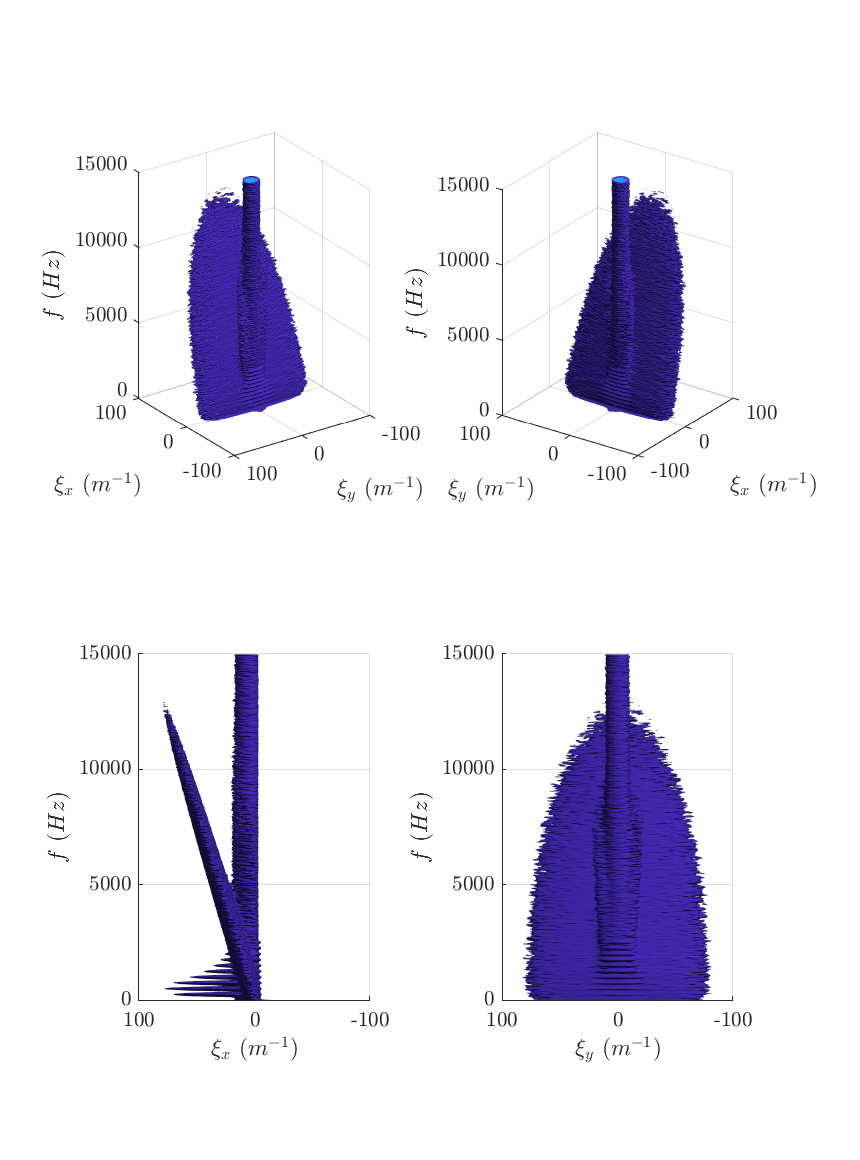
\includegraphics{../matlab/04_basic_filtering/filter_downstream.eps}
  \caption{Dispersion isosurface of the synthetic wavefront with a downstream filter in place (left) and unfiltered (right).}
  \label{fig:04_filter_downstream}
\end{figure}
All of the upstream traveling disturbances are removed and the disturbances at $\xi_x=0$ m$^{-1}$ are significantly reduced.
Some of the stationary modes remain while only the acoustic and vibration signals that are propagating in the direction of flow remain.
The aero-optical signal is clipped slightly at $\xi_x=0$ due to the spatial width of the signal.
The ratio of the time-averaged spatial-RMS of the filtered signal when compared to the aero-optic only signal was 1.24 while the unfiltered ratio was 1.53.
When the filter was applied to only the aero-optic signal the ratio was 0.96.
This filter method is will retain any disturbance that is traveling of flow such that any contamination moving in this direction will be retained.
Even with an ideal filter there is some slight attenuation of the aero-optical signal due to signal having some spectral width that crosses into upstream-moving portion of the dispersion plot.


\section{Velocity Filtering}
The dispersion plot shows flow structures that are traveling at a given speed as having a constant slope in a given direction over a large frequency range.
A plane in the dispersion plot can be used to measure a flow structures velocity in both $x$ and $y$-directions.
The distance from any given point in the dispersion plot to a plane described by the velocities $v_x$ and $v_y$
\begin{equation}
  d = \frac{|v_x\xi_x+v_y\xi_y-f|}{\sqrt{v_x^2+v_y^2+1}} \textrm{.}
  \label{eqn:04_dist_point_2_plane}
\end{equation}
A low-pass or high-pass filter can then be used to retain only disturbances that are traveling at that velocity or to exclude those disturbances respectively.

A low-pass velocity-filter of the synthetic wavefront is shown Figure \ref{fig:04_filter_velocity}.
\begin{figure}
  \centering
  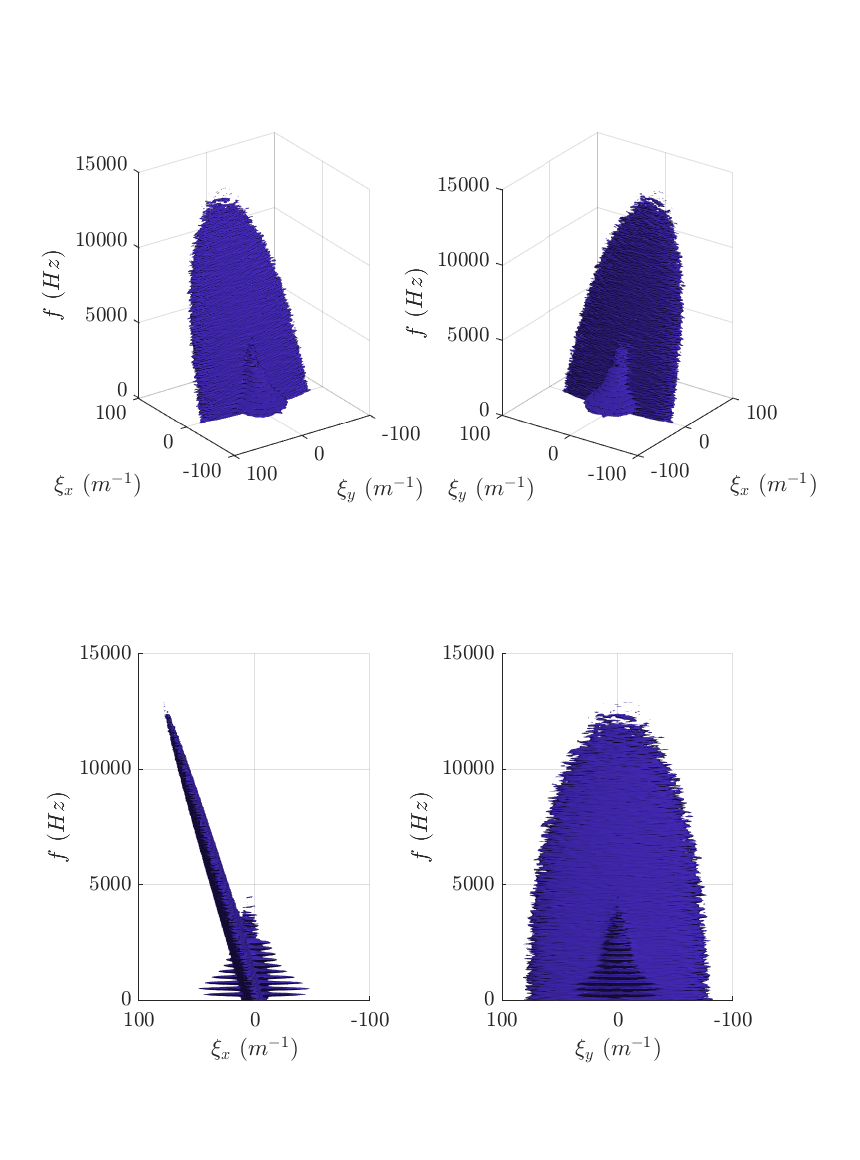
\includegraphics{../matlab/04_basic_filtering/filter_velocity.eps}
  \caption{Dispersion isosurface of the synthetic wavefront with a low-pass velocity-filter in place (left) and unfiltered (right).}
  \label{fig:04_filter_velocity}
\end{figure}
The filtered dispersion plot (left) shows primarily only the aero-optic signal remains with some additional low-frequency content from the blade-passing frequency and harmonic disturbances as well as some stationary and acoustic disturbances.
The ratio of the time-averaged spatial-RMS relative to that of the aero-optical only signal went from 1.53 in the unfiltered case to 1.01 in the filtered case.
This method can provide a very effective way in quickly estimating the clean spatial-RMS of a contaminated wavefront.

Another use of the synthetic wavefront is measuring the speed of a broadband disturbance such as the aero-optical signal of a boundary layer.
This is done by finding the velocity that maximizes the output spatial-RMS of the velocity filter, see Figure \ref{fig:04_filter_velocity_measure}.
\begin{figure}
  \centering
  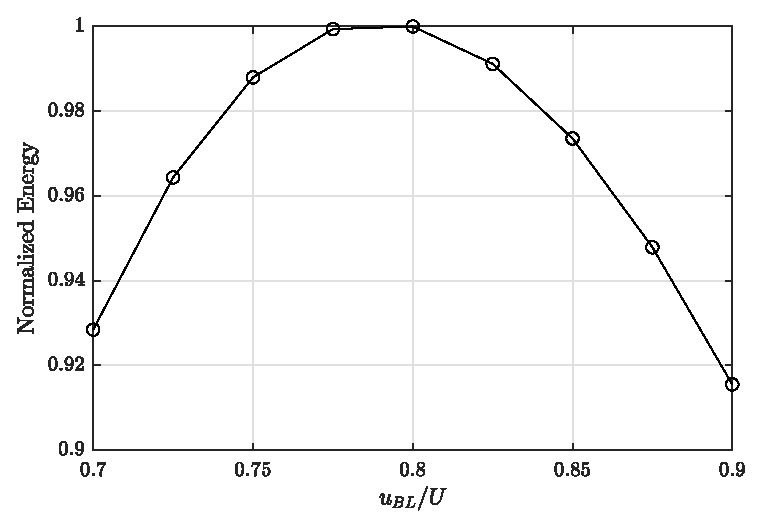
\includegraphics{../matlab/04_basic_filtering/filter_velocity_measure.eps}
  \caption{Velocity low-pass filter used to determine the mean disturbance velocity.  The maximum value corresponds with the actual value used in the creation of the synthetic wavefront.}
  \label{fig:04_filter_velocity_measure}
\end{figure}
In this case boundary layer speed was determined to be 163 m/s which corresponds to the design velocity of the synthetic signal of $0.8U$.
If the velocity range used is to large, a false result can be obtained due the inclusion of disturbance structures not related to the aero-optical signal.
For signals that have a mean-velocity component that is not aligned with an axis both velocity components can be varied as shown in Figure \ref{fig:04_filter_velocity_real}.
\begin{figure}
  \centering
  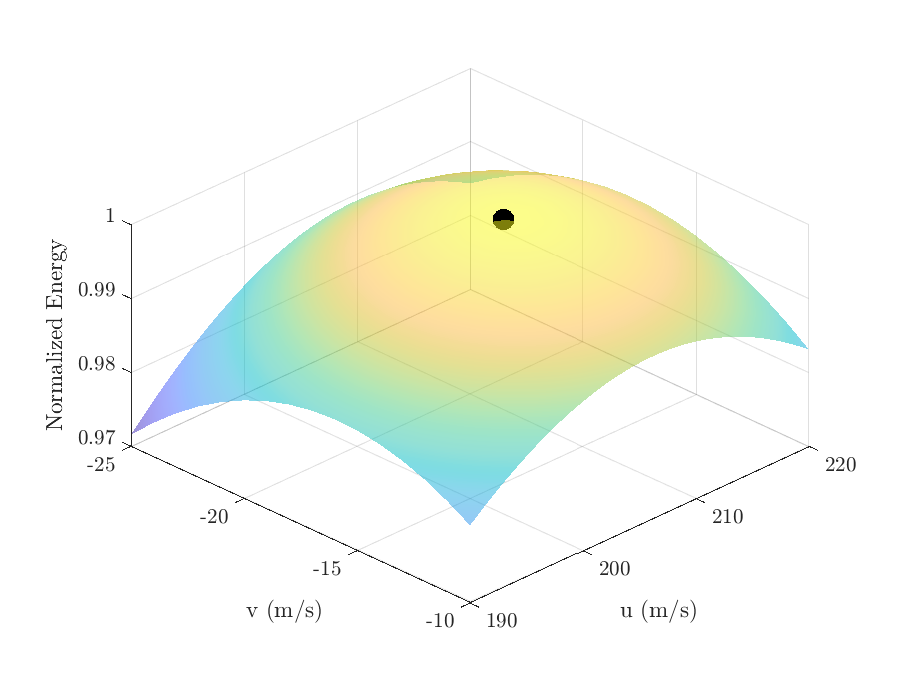
\includegraphics{../matlab/04_basic_filtering/filter_velocity_real.eps}
  \caption{Velocity low-pass filter used to determine the mean disturbance velocity of measured data presented in Figure \ref{fig:04_dispersion_real}.  The velocity in the x-direction was measured to be 207 m/s and -17 m/s in the y-direction.}
  \label{fig:04_filter_velocity_real}
\end{figure}
In this case a variable low-pass velocity filter was employed with a high-pass spatial filter operating in the radial direction.
This helped eliminate some of the low-frequency stationary disturbances as well as some of the disturbances related to the blade-passing frequency.
The velocity was measured using the optical disturbances in the dispersion plot to be approximately 207 m/s in the x-direction and -17 m/s in the y-direction.

% !TEX root = catron-dissertation.tex
\epstopdfsetup{outdir=./images/05_advanced_filtering/}

\chapter{Advanced Wavefront Filtering Techniques}


\appendix
% !TEX root = catron-dissertation.tex
\chapter{Sample Code}

\lstinputlisting[label=code:sc_simpleSXX, caption={A simple function for computing the power spectra for vector \lstinline{x} given an arbitrary windowing function.}, language=Matlab]{../matlab/00_functions/simpleSXX.m}

\lstinputlisting[label=code:sc_simpleSXXn, caption={A simple function for computing the dispersion or n-dimensional power spectra of \lstinline{x} given an arbitrary windowing function.}, language=Matlab]{../matlab/00_functions/simpleSXXn.m}

\lstinputlisting[label=code:sc_synthetic_wavefront, caption={MATLAB code used to generate the synthetic wavefront used in Chapter \ref{chap:wavefront_filtering}.}, language=Matlab]{../matlab/05_synthetic_wavefront/synthetic_wavefront.m}

\lstinputlisting[label=code:sc_basic_wavefront_filters, caption={MATLAB code used to filter wavefronts in Chapter \ref{chap:wavefront_filtering}.}, language=Matlab]{../matlab/00_functions/WFfilter.m}

% \lstinputlisting[label=code:sc_spatial_window, caption={MATLAB code used to generate a spatial windowing function for an arbitrary two-dimensional mask.}, language=Matlab]{../matlab/00_functions/createSpatialWindow.m}

% \lstinputlisting[label=code:wfdispersion, caption={Dispersion analysis code}, language=Matlab]{../matlab/00_functions/WFdispersion.m}


\backmatter
\bibliographystyle{nddiss2e}
\bibliography{80_references.bib}

\end{document}
